% !TeX spellcheck = it_IT
% !TeX root = thesis-main.tex
\documentclass[12pt,a4paper,openright,twoside]{book}
\usepackage[italian]{babel}
\usepackage[hyperfootnotes=false]{hyperref}
\usepackage{disi-thesis}
\usepackage[acronym,toc]{glossaries}
\usepackage{code-lstlistings}
\usepackage{notes}
\usepackage{shortcuts}
\usepackage{float}
\usepackage{pgfplots}

\tolerance=1000
\pgfplotsset{compat=1.18}

\newcommand{\acknowledgementsname}{Riconoscimenti}
\renewcommand{\chaptername}{Capitolo} % Per i capitoli
\renewcommand{\bibname}{Bibliografia} % Per la bibliografia
\renewcommand{\contentsname}{Indice}  % Per il sommario
\renewcommand{\listfigurename}{Elenco delle figure}
\renewcommand{\listtablename}{Elenco delle tabelle}
\newcommand{\itemdef}[1]{\item \textbf{#1}}
\newcommand{\class}[1]{\texttt{#1}}
\newcommand{\cs}{C\# }

\usepackage{booktabs} % Per una tabella più professionale
\usepackage{graphicx} % Per la gestione delle dimensioni della tabella
\usepackage{xcolor} % Per colorare le righe

\glsdisablehyper

\pagenumbering{roman}



\school{\unibo}
\programme{Corso di Laurea in Ingegneria e Scienze Informatiche}
\title{ClientShield: Implementazione di un Servizio Windows per la Sicurezza DNS}
\author{Federico Diotallevi}
\date{\today}
\subject{Programmazione ad Oggetti}
\supervisor{Prof.\ Viroli Mirko}
\cosupervisor{Dott.\ Nicolas Farabegoli}
\session{IV}
\academicyear{2023\ -\ 2024}

\newacronym{DoH}{DoH}{DNS over HTTPS}
\newacronym{DoT}{DoT}{DNS over TLS}
\newacronym{DNS}{DNS}{Domain Name System}
\newacronym{AI}{AI}{Intelligenza Artificiale}
\newacronym{PoC}{PoC}{Proof of Concept}
\newacronym{AGID}{AGID}{Agenzia per l'Italia Digitale}
\newacronym{VPN}{VPN}{Virtual Private Network}
\newacronym{HTTPS}{HTTPS}{HTTP Secure}
\newacronym{ISP}{ISP}{Internet Service Provider}
\newacronym{OS}{OS}{Sistema Operativo}
\newacronym{SRP}{SRP}{Single Responsibility Principle}
\newacronym{MVP}{MVP}{Model-View-Presenter}
\newacronym{MVC}{MVC}{Model-View-Controller}
\newacronym{WPF}{WPF}{Windows Presentation Foundation}
\newacronym{IDE}{IDE}{ambiente di sviluppo integrato}
\newacronym{WSL}{WSL}{Windows Subsystem for Linux}


\mainlinespacing{1.241} % line spacing in mainmatter, comment to default (1)

\begin{document}

\frontmatter
\frontispiece

\renewcommand{\abstractname}{Sommario}
\begin{abstract}

Lo sviluppo della tecnologia cresce sempre più velocemente: il costante incremento della potenza computazionale e l'avvento dell'intelligenza artificiale hanno consentito lo sviluppo di malware sempre più sofisticati, aumentando i rischi che gli utenti corrono semplicemente navigando sul web.
Questa tesi si inserisce nell'ambito della sicurezza in rete, trattando di internet filtering, cioè la possibilità di filtrare il traffico in rete negando l'accesso a siti potenzialmente pericolosi.

L'obiettivo di questo progetto è lo sviluppo di un software che sia facilmente installabile su un dispositivo Windows e filtri tutte le richieste web effettuate.
Si vuole offrire la possibilità ad un amministratore di rete di attivare e disattivare la protezione del dispositivo da remoto, decidendo eventualmente anche quali categorie di siti bloccare.

Per lo sviluppo è stata fondamentale la collaborazione con FlashStart, azienda di riferimento nel mercato italiano per quanto riguarda il filtraggio DNS.
Il software è stato sviluppato in contesto aziendale come prototipo e sfrutta ampiamente le soluzioni di filtraggio aziendali.
Ciò ha facilitato la gestione delle categorie e dell'effettivo filtraggio DNS, permettendo al progetto di focalizzarsi sulla cattura e redirezione del traffico internet del dispositivo verso i server gestiti da FlashStart.
\end{abstract}

\begin{dedication}
Ai miei fratelli e alle mie sorelle,\\
nella speranza che sempre assieme\\
affronteremo le difficoltà\\
e festeggeremo i nostri successi.
\end{dedication}

%----------------------------------------------------------------------------------------
\tableofcontents   
%\listoffigures     % (optional) comment if empty
%\lstlistoflistings\ % (optional) comment if empty
%----------------------------------------------------------------------------------------

%----------------------------------------------------------------------------------------

%---------------------------------------------------
% INTRODUZIONE
%---------------------------------------------------

\chapterWithoutNumber{Introduzione}
\phantom{Introduzione}
\label{chap:introduzione}
%----------------------------------------------------------------------------------------

Navigare in rete è senz'altro una delle attività più diffuse al giorno d'oggi in tutto il mondo.
La quantità di informazioni a cui si può accedere è pressoché infinita e, soprattutto, a disposizione di chiunque.

La digitalizzazione delle risorse è ormai diventata essenziale per qualsiasi realtà, dal settore pubblico a quello privato.
Tuttavia, tale pratica espone inevitabilmente al rischio che documenti,
dati e informazioni sensibili diventino obiettivo di attacchi informatici.
A conferma di ciò, il recente rapporto \cite{clusit2024-sicurezza} evidenzia come gli attacchi informatici gravi a livello globale siano passati,
in media, da 4.5 a 9 al giorno in soli cinque anni.
Secondo il rapporto, gli incidenti critici sono aumentati dal 47\% all'81\% del totale e,
in Italia, il 58\% degli attacchi è costituito da malware, phishing e social engineering.

Con il recente e rapidissimo sviluppo dell' \gls{AI} il campo dell'Internet Filtering ha subito un vera e propria rivoluzione.
I nuovi modelli di Machine Learning sono capaci di analizzare e identificare con precisione siti malevoli,
grazie anche ai giganteschi volumi di dati di cui dispongono.
Questi sistemi riescono a riconoscere tecniche di phishing e malware avanzate, anche quando progettate per eludere i metodi di rilevamento tradizionali.

Questa tesi si colloca in questo contesto e si pone l'obiettivo di sviluppare un software prototipale per il filtraggio internet sul computer di installazione.
Il lavoro illustrerà dettagliatamente tutte le fasi di analisi, progettazione e sviluppo del progetto.

Data la necessità di interazione con componenti specifici del sistema operativo,
il software è stato sviluppato esclusivamente per Windows, con l'obiettivo di creare un servizio di sistema.

\section*{Struttura della Tesi}

La tesi si articola in 4 capitoli principali, che descrivono le diverse fasi della realizzazione del progetto, in particolare:



\begin{itemize}

    \itemdef{Capitolo 1 (Contesto)}: in questo capitolo si tratta in maniera approfondita il problema affrontato dalla tesi.
    Viene analizzato il software attualmente presente in FlashStart e le motivazioni che inducono alla necessità di un nuovo sviluppo.
    
    \itemdef{Capitolo 2 (Requisiti)}: in questo capitolo vengono affrontati casi d'uso e requisiti, analizzando il funzionamento e la percezione del progetto dal punto di vista dell'utente.
    
    \itemdef{Capitolo 3 (Analisi e progettazione)}:
    in questo capitolo viene descritta la fase di analisi e progettazione del sistema,
    illustrandone in particolare l'architettura e i pattern utilizzati, evidenziando in che modo il software ne tragga guadagno.
    
    \itemdef{Capitolo 4 (Implementazione)}:
    in questo capitolo viene descritta l'intera fase di sviluppo, riportando linguaggi, librerie e tecnologie utilizzate per l'implementazione del software.

\end{itemize}

\mainmatter

%---------------------------------------------------
% CAPITOLO 1
%---------------------------------------------------
\chapter{Contesto}
\label{chap:contesto}

\section{Internet Filtering}

Il caso di studio oggetto di questa tesi è un software prototipale, che si inserisce nell'ambito dell'Internet Filtering.
Per Internet Filtering si intende un sistema di monitorazione, controllo e limitazione dell'accesso alle risorse online, basato su criteri predefiniti.

Una tecnologia di questo tipo risulta particolarmente utile ad aziende, scuole ed enti pubblici.
Tramite questa pratica è infatti possibile effettuare controlli sul contenuto delle pagine web, limitando o impedendo l'accesso a siti contenenti malware o, eventualmente, contenuti indesiderati (ad esempio siti di scommesse, pornografia, droghe...).
Risulta evidente fin da subito che, per garantire un filtraggio di contenuti preciso ed efficace, sia necessaria un'attenta analisi delle pagine web, evitando di correre il rischio di impedirne immotivatamente l'accesso.

Questa tesi è svolta come progetto in collaborazione con FlashStart, leader italiana per quanto riguarda il filtraggio \gls{DNS}.
Un server \gls{DNS} è un sistema che permette di tradurre nomi di domini leggibili da un umano, in indirizzi interpretabili da dei computer per connettersi tra loro.
Il filtraggio si basa proprio su questo principio: quando si accede ad un sito web attraverso un browser qualsiasi, il computer interrogherà un server \gls{DNS} per ottenere l'indirizzo attraverso cui sia possibile accedere al sito.
Con un'apposita configurazione, si può indurre il \gls{DNS} a bloccare la risoluzione di pagine web malevoli o riportanti contenuti non graditi.
FlashStart offre un servizio \gls{DNS} configurabile, attraverso cui è possibile definire delle categorie di contenuti da bloccare.
I server dell'azienda aggiornano continuamente la lista delle categorie bloccate, facendo largo uso di \gls{AI} per garantire rapido aggiornamento (in risposta alla nascita di nuovi siti) ed alta precisione.
Quando un utente, utilizzando un computer protetto dal servizio di FlashStart, tenta di accedere ad un sito appartenente ad una delle categorie bloccate, il \gls{DNS} risponderà alla richiesta di risoluzione del nome con l'indirizzo di una pagina indicante i motivi del blocco, al posto di quella richiesta.

\section{Obiettivi del Progetto}
\label{sec:obiettivi-progetto}

Il filtraggio \gls{DNS} può essere implementato in diverse modalità, di seguito le principali:

\begin{itemize}
	\item \textbf{A livello di rete:} applicato direttamente dall'\gls{ISP}\footnote{
		Un \gls{ISP} è un fornitore che offre connettività alla rete, consentendo ai suoi utenti di accedere a Internet. Gli ISP possono anche fornire servizi aggiuntivi, come, appunto, sicurezza informatica e filtraggio.}, blocca l'accesso a domini malevoli prima che le richieste raggiungano la rete locale.  
	\newline \textit{Esempio: un'azienda utilizza un servizio \gls{DNS} filtrato fornito dal proprio \gls{ISP} per impedire l'accesso a siti malevoli su tutta la rete aziendale.}
	
	\item \textbf{A livello di router:} il router funge da punto di controllo, utilizzando un server DNS con filtraggio per impedire l'accesso a contenuti non autorizzati. Tutti i dispositivi connessi alla rete collegata al router beneficiano automaticamente della protezione.
	\newline \textit{Esempio: un istituto scolastico configura il proprio router con un DNS appositamente configurato per impedire l'accesso a siti per adulti e social network bloccandoli per gli studenti.}
	
	\item \textbf{A livello di endpoint:} il filtraggio DNS è applicato direttamente sui dispositivi tramite configurazione manuale o software specifici, garantendo protezione anche fuori dalla rete aziendale o domestica.  
	\newline \textit{Esempio: un dipendente che lavora da remoto utilizza un client DNS sicuro sul proprio laptop per proteggersi dalle minacce.}
\end{itemize}

FlashStart offre prodotti per tutte le suddette modalità, tuttavia questo progetto prende in esame soltanto la terza tipologia di protezione \gls{DNS}, ossia il filtraggio a livello di endpoint.
Nel periodo tra il 2019 e il 2021 le aziende italiane, così come quelle di tutto il mondo, hanno dovuto affrontare la necessità dell'impiego del lavoro da remoto.
Se da una parte tale pratica rappresenta un'opportunità per i lavoratori, che ne guadagnano in flessibilità, dall'altra espone l'azienda a nuovi rischi.
A dimostrazione di ciò, proprio nel 2020 è stato emanato dall'\gls{AGID} il vademecum \cite{AgID2020}, cioè una serie di undici raccomandazioni che offrono linee guida per garantire la sicurezza del lavoro da remoto.

In effetti, un dispositivo che esce dall'azienda, ambiente potenzialmente controllato e protetto, diventa un rischio.
Un dipendente potrebbe involontariamente navigare in siti di phishing e malware o connettersi a reti Wi-Fi infette, esponendo l'azienda al rischio di furti o compromissione di dati.
Obiettivo fondante di questa tesi è lo sviluppo di un software facilmente installabile su un computer Windows, che consenta una protezione efficace e completa ai dispositivi desktop che escono dalla rete aziendale.
Tale progetto dovrà filtrare la connessione dell'endpoint remoto, bloccando l'accesso a siti pericolosi, come virus e frodi, ma anche a contenuti indesiderati e distrazioni sul lavoro, come social network o videogiochi.

\section{Contesto Aziendale}

FlashStart offre già un software di protezione da malware e contenuti indesiderati dedicato ad endpoint remoti: ClientShield.
Tale prodotto rappresenta un'estensione del filtro aziendale, fornendo lo stesso tipo di protezione, configurabile attraverso la medesima piattaforma cloud da parte di un amministratore di rete.

Allo stato dell'arte il prodotto utilizza una \gls{VPN}, per stabilire una comunicazione sicura con i server di FlashStart.
Ciò garantisce che il dispositivo possa inviare e ricevere non soltanto le informazioni sul prodotto, ma anche richieste \gls{DNS}, generalmente trasmesse in chiaro, in modo totalmente criptato.

L'esigenza di aggiornamento del software deriva dalla volontà di FlashStart di integrare il protocollo \gls{DoH}, descritto in \cite{RFC8484}, nei suoi prodotti.
Rispetto ad una classica \gls{VPN}, \gls{DoH} sfrutta la crittografia asimmetrica, implementata dal protocollo \gls{HTTPS}, per garantire autenticazione, confidenzialità e integrità delle richieste \gls{DNS}.

Il vantaggio che FlashStart trae da entrambi i protocolli è essenzialmente il medesimo: proteggere le comunicazioni \gls{DNS} tramite la crittografia, evitando la possibilità di attacchi dovuti alla trasparenza delle informazioni.
La differenza principale tra i due approcci è che una \gls{VPN} cripta il traffico di rete nella sua interezza, mascherando anche l'indirizzo IP del dispositivo, mentre \gls{DoH} si concentra esclusivamente sulla protezione delle richieste \gls{DNS}.

Per un'azienda come FlashStart, specializzata in filtraggio \gls{DNS}, mascherare l'indirizzo IP di un endpoint non è una funzionalità totalmente rilevante per l'erogazione del suo servizio.
L'adozione del protocollo \gls{DoH} consente quindi di ottenere la riservatezza necessaria per la comunicazione con il \gls{DNS}, eliminando la necessità di un'infrastruttura \gls{VPN} dedicata e riducendo l'overhead complessivo del sistema.

La novità principale del software prototipale illustrato in questa tesi, è dunque quella di fornire una soluzione per la transizione dalla tecnologia \gls{VPN}, all'adozione del protocollo \gls{DoH}.
Di fondamentale importanza è inoltre l'analisi e la valutazione di soluzioni architetturali atte a garantire la naturale evoluzione del software, facilitando l'introduzione di nuove funzionalità.


%---------------------------------------------------
% CAPITOLO 2
%---------------------------------------------------

\chapter{Analisi dei Requisiti}
\label{chap:analisi-dei-requisiti}

\section{Scopo del sistema e analisi del dominio}

L'analisi del dominio è un punto chiave per quanto riguarda lo sviluppo software.
Tale fase permette di comprendere il contesto in cui il software opera, gli attori principali ed i loro scopi.
In questo progetto l'analisi del dominio è risultata molto rapida e diretta, in quanto il prodotto è stato sviluppato con un'azienda del settore informatico, permettendo fin da subito l'utilizzo di un linguaggio tecnico.

Come già introdotto nella sezione \ref{sec:obiettivi-progetto}, il contesto in cui opera l'applicazione è quello della sicurezza informatica.
Il fine ultimo di ClientShield è di fornire una soluzione di filtraggio \gls{DNS} avanzata, che consenta un'efficace protezione ad un dispositivo che naviga al di fuori di una rete protetta.
L'interazione col software coinvolgerà in particolare:

\begin{itemize}
	\item \textbf{Utente finale:} cioè l'utilizzatore del dispositivo da proteggere, il quale navigherà normalmente in internet, utilizzando un browser ed inviando naturalmente richieste \gls{DNS}.
	
	\item \textbf{Amministratore di rete:} il cliente FlashStart, responsabile dell'installazione e configurazione del software sul dispositivo attraverso la chiave fornita sulla piattaforma cloud. 
	Tramite l'applicativo online potrà gestire le policy di filtraggio, aggiungendo o rimuovendo siti specifici o intere categorie di contenuti da bloccare.

	\item \textbf{Server FlashStart:} riceveranno le richieste \gls{DNS} effettuate dal dispositivo protetto e le risolveranno applicando i filtri configurati dall'amministratore di rete.
\end{itemize}
Il software dovrà operare in modo tale da rendersi completamente trasparente all'utente finale, il quale non dovrebbe percepire alcuna differenza durante la normale navigazione.

\section{Requisiti funzionali}

Il progetto prevede lo sviluppo di un'implementazione prototipale, ciò implica che le funzionalità del software trattate in questa tesi rappresentino un sottogruppo delle capacità che dovrà avere il sistema.
Tuttavia, poiché il risultato dello studio mira a gettare delle solide basi per una futura implementazione business di ClientShield, di seguito verranno elencati i requisiti del software nella sua interezza.
Una visione complessiva, infatti, permette di valutare fin da subito la possibilità di una futura integrazione delle funzioni aggiuntive, consentendo un'analisi più efficace.

Nella sua implementazione prototipale, ClientShield dovrà:

\begin{itemize}
	\item \textbf{Redirezionare le richieste \gls{DNS}:}
	l'applicazione catturerà tutto il traffico \gls{DNS} del dispositivo su cui è installata.
	Tutte le richieste devono essere redirezionate ai server FlashStart, sfruttando il protocollo \gls{DoH}.
	La risoluzione dei domini deve essere effettuata dai server aziendali, ClientShield agirà da client \gls{DoH}, facendo in modo di impedire la possibilità di \gls{DNS} leak\footnote{\textbf{DNS leak} si verificano quando le richieste \gls{DNS} non sono cifrate e vengono trasmesse in chiaro.  
		In questa condizione, un attaccante o qualsiasi entità che intercetti il traffico può monitorare i siti visitati dall'utente, compromettendo la privacy della navigazione.}.

	
	\item \textbf{Permettere la registrazione di un dispositivo localmente:}
	dopo l'installazione del software, chiunque disponga di una valida chiave di registrazione, può registrare il dispositivo.
	Per effettuare tale operazione saranno richiesti:
	\begin{itemize}
		\item \textit{chiave di registrazione:} ottenibile tramite un profilo cloud con la corretta licenza.
		\item \textit{nome del dispositivo:} una qualsiasi stringa che faciliti l'identificazione dell'endpoint ad un amministratore di rete.
	\end{itemize}
	Al termine della fase di registrazione, se avvenuta con successo, la protezione dovrà essere attivata e il dispositivo sarà visibile sulla piattaforma cloud.
	
	
	\item \textbf{Abilitare/disabilitare la protezione localmente:}
	accedendo all'applicazione, qualora la protezione sia disattivata, si dovrà offrire la possibilità di attivarla.
	Viceversa, se la protezione è attiva, l'utente avrà la possibilità di disattivarla inserendo un PIN.
	Tale codice è un numero intero presente sulla piattaforma cloud e dunque visualizzabile soltanto da un amministratore di rete.
	
	\item \textbf{Controllare lo stato:}
	l'applicazione dovrà periodicamente connettersi ai server FlashStart per verificare lo stato della protezione.
	Questa operazione nell'implementazione prototipale ha la funzione di verificare che il dispositivo sia ancora registrato sul cloud.
	La cancellazione dell'endpoint attraverso la piattaforma cloud, determinerà la disattivazione della protezione e la richiesta di una nuova registrazione.
	
	\item \textbf{Attivarsi automaticamente al riavvio:}
	se l'endpoint è già stato registrato, l'applicazione dovrà garantire il corretto funzionamento della protezione anche al riavvio.
	Ciò vuol dire che, all'accensione del dispositivo non dovrà essere necessaria, una nuova registrazione.
	ClientShield ricorderà le credenziali attive prima dello spegnimento, riattivando automaticamente la protezione all'accensione con le stesse.
	
\end{itemize}
Queste funzionalità costituiscono il comportamento complessivo del prototipo sviluppato in questo progetto.
L'obiettivo essenziale è dunque garantire la protezione del dispositivo, fungendo da intermediario tra l'endpoint e i server di FlashStart.
Con lo scopo di descrivere in modo semplice l'interazione tra utente, ClientShield e server \gls{DNS} FlashStart è stato realizzato il diagramma in figura \ref{fig:interazione-utente-software-server}.

\begin{figure}[H]
	\centering
	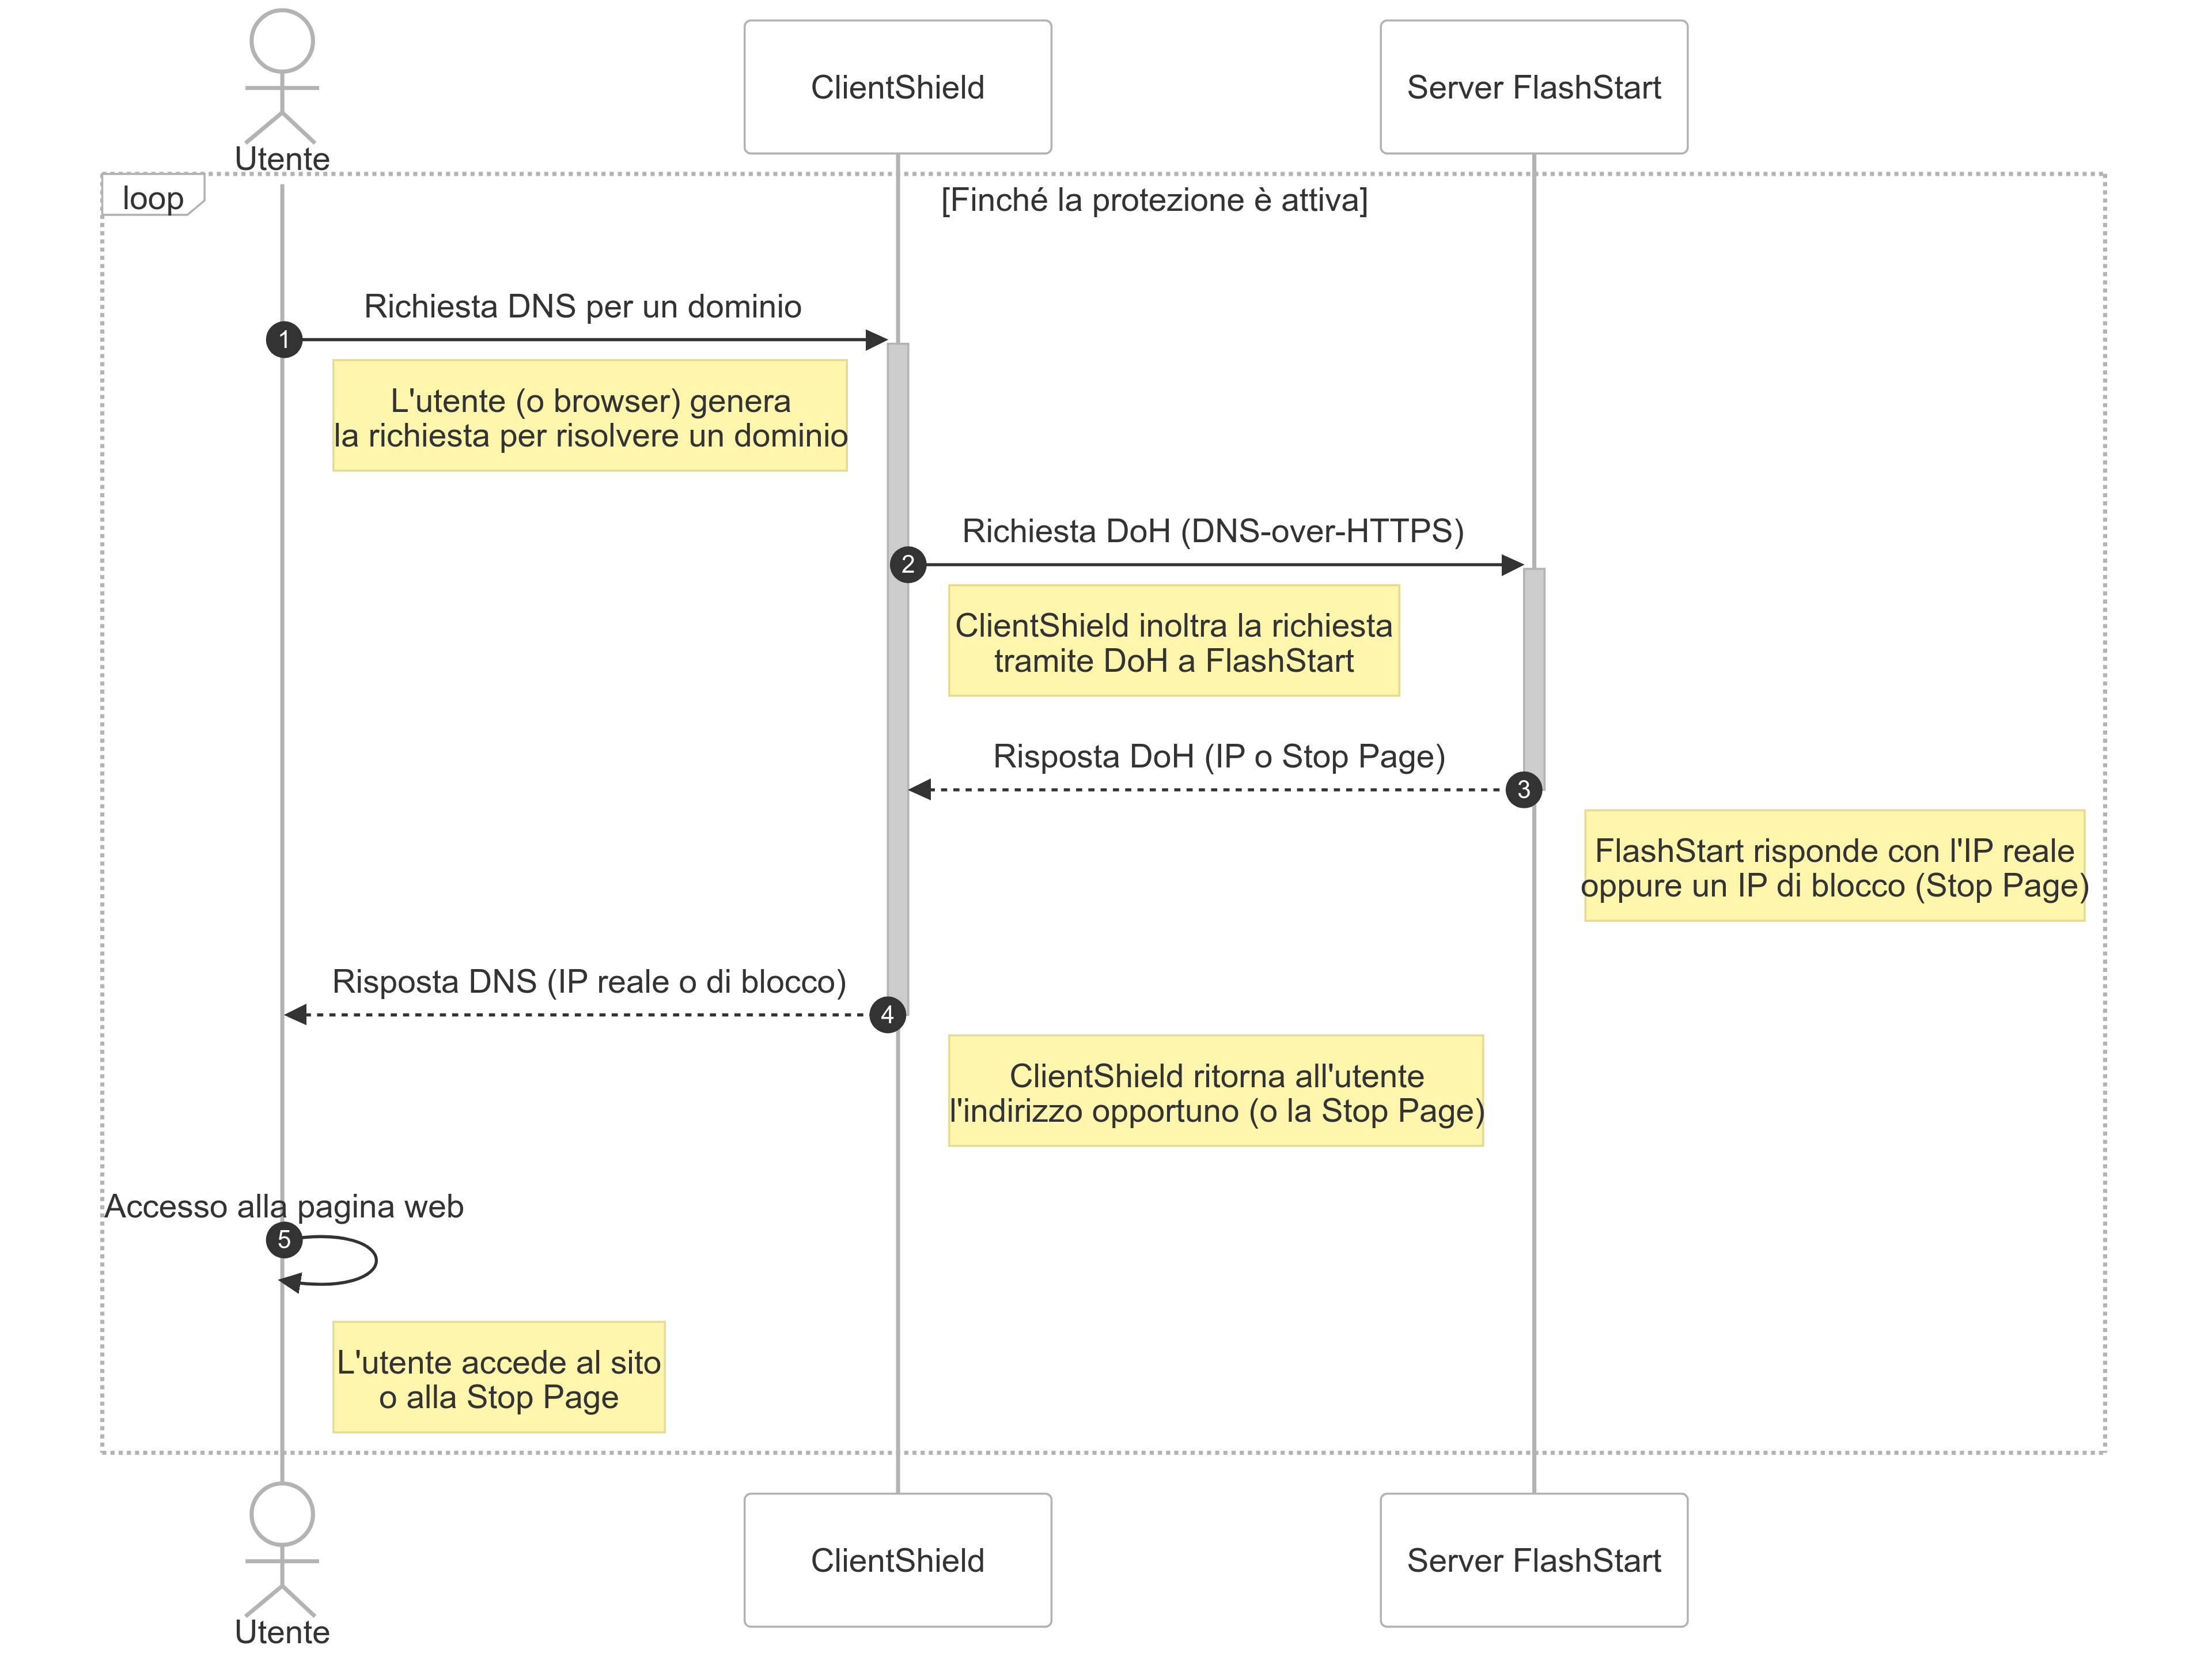
\includegraphics[width=1.0\textwidth]{figures/schema-utente-software-server.png}
	\caption{interazione tra utente, software e server FlashStart}
	\label{fig:interazione-utente-software-server}
\end{figure}

Come precedentemente anticipato, la versione business dell'applicazione garantirà una serie di funzioni minori in più, di seguito riportate:

\begin{itemize}
	
	\itemdef{Blocco remoto della protezione:}
	deve essere possibile disattivare la protezione da remoto, questa funzione può essere utilizzata sia dall'amministratore di rete, attraverso la piattaforma cloud, sia direttamente dai server FlashStart.
	Durante i controlli di stato periodici, infatti, verrà verificata la validità della licenza e, se non risultasse valida, la protezione verrà disattivata automaticamente, impedendo qualsiasi tentativo di riattivazione locale.
	
	\itemdef{Invio di notifiche:}
	durante la registrazione sarà possibile decidere di ricevere alcune notifiche dall'applicazione.
	Se attivate, il dispositivo riceverà soltanto le notifiche riguardanti lo stato della protezione del dispositivo, ad esempio licenza scaduta o disabilitazione remota.
	
	\itemdef{Applicazione unbranded:} 
	l'applicazione prima della registrazione dovreb-be avere un nome generico e non presentare alcun logo.
	Dopo la registrazione dovrà essere possibile ottenere informazioni sull'acquirente, come il nome scelto per il software e il logo da applicare.
	L'interfaccia grafica dell'applicazione dovrà adattarsi alle informazioni ottenute durante la registrazione.
	
	\itemdef{Controllo di stato periodico:}
	questa operazione è già presente in parte nell'implementazione prototipale, tuttavia nello sviluppo business dovrà reperire più informazioni.
	I dati supplementari, come ad esempio:
	\begin{itemize}
		\item informazioni sul blocco remoto
		\item nome e logo dell'acquirente
		\item cambio di impostazioni sulle notifiche
	\end{itemize}
	permetteranno l'implementazione delle funzionalità aggiuntive sopra riportate.

\end{itemize}
Come si può notare, le funzionalità business rappresentano più che altro un'estensione di funzioni già presenti nel modello prototipale.
Con una corretta analisi del software, dunque, dovrebbe essere possibile aggiungere tutte le funzionalità supplementari al sistema descritto in questa tesi senza particolari sforzi.

\section{Requisiti non funzionali}

Dopo aver definito in dettaglio \textit{cosa} deve fare ClientShield, è altrettanto importante stabilire \textit{come} debba farlo.
Oltre ai requisiti funzionali del sistema, infatti, il progetto prevede anche dei requisiti non funzionali, che mirano a garantire un livello qualitativo adeguato al sistema.
Questa categoria di requisiti ha l'obiettivo di soddisfare un potenziale cliente.
L'aderenza ad essi dovrebbe trasmettere la professionalità di FlashStart, garantendo un'esperienza di utilizzo piacevole per gli utilizzatori finali.

\subsection*{Semplicità}

Di fondamentale importanza è rendere il sistema semplice: rapido da installare e facile da configurare.  
FlashStart ha esplicitamente sottolineato quanto questo requisito sia cruciale per garantire la qualità del software.
La richiesta è naturalmente intuitiva: un'installazione e una configurazione rapide non solo migliorano l’esperienza dell’utente, ma rendono il software più facilmente integrabile nei diversi contesti aziendali.  
L'automatizzazione completa del processo di installazione consente agli amministratori di rete di implementare ClientShield senza difficoltà, ottimizzando i tempi e riducendo il rischio di errori nella configurazione.  

\subsection*{Efficienza}

Anche nello sviluppo prototipale, ClientShield dovrebbe garantire un'efficienza tale da risultare totalmente trasparente all'utente.
L'obiettivo è limitare qualsiasi impatto sulla navigazione, un utente qualunque del dispositivo dovrebbe potersi scordare della presenza di un filtro.
Ciò implica una rapida gestione delle richieste \gls{DNS}, consentendo una veloce risoluzione dei domini, limitando di conseguenza i tempi di caricamento delle pagine web.

Questo requisito è favorito dall'abbandono dell'utilizzo di una \gls{VPN} in favore del protocollo \gls{DoH} e dalla velocità generale dei server di FlashStart, che, a febbraio 2025, risulta essere il \gls{DNS} più veloce al mondo secondo \cite{DNSPerf2025}.

\subsection*{Resilienza}

Per garantire la corretta protezione del dispositivo, il servizio di filtraggio dovrebbe poter essere disattivato esclusivamente da un amministratore del dispositivo.
Ciò vuol dire che ClientShield dovrà assicurare il funzionamento continuo della protezione in qualsiasi condizione, anche nel caso in cui l'utente tenti di disattivare il filtro.
È requisito essenziale per il software fare in modo che nessuna operazione effettuata da utenti senza privilegi amministrativi, come il banale cambio di rete, possa interrompere la protezione.

\section{Casi d'uso}
\label{sec:casi-d-uso}

Allo scopo di descrivere in modo dettagliato il comportamento atteso del software, vengono di seguito riportati anche i casi d'uso del sistema.
Ciascun caso d'uso rappresenta una specifica interazione tra gli attori e ClientShield, chiarificando le azioni che possono essere eseguite e le risposte da parte dell'applicazione.
Questa visione è particolarmente utile, perché pone l'attenzione sull'utente, evidenziando come interagirà con ClientShield e cosa percepirà in seguito ad ogni possibile azione eseguita.
Di seguito sono riportati i principali casi d'uso del prototipo:

\begin{itemize}
	
	\item \textbf{Utente avvia l'applicazione:}
	all'avvio dell'applicazione se il dispositivo non risulta registrato, l'utente verrà indirizzato ad una schermata di registrazione.
	Se invece l'utente è già registrato e la protezione è disattivata, allora verrà offerta la possibilità di attivarla.
	Viceversa, se è già registrato e la protezione è attiva, deve essere disponibile un'opzione per disattivarla.
	
	\item \textbf{Registrazione:}
	per registrarsi l'utente dovrà inserire i campi richiesti (chiave di profilo e nome del dispositivo).
	Se la registrazione ha avuto successo la protezione deve essere attivata, iniziando subito a filtrare le richieste \gls{DNS}.
	Per la comunicazione con i server FlashStart sarà necessario un codice utente univoco, ottenibile come risposta alla fase di registrazione.
	In caso di errore, la causa deve essere visibile dall'utente, che potrà ritentare.
	
	\item \textbf{Disattivazione protezione:}
	per disattivare la protezione tramite l'applicazione sarà necessario l'inserimento di un codice PIN.
	Il PIN è un numero intero visualizzabile dalla piattaforma cloud e deve essere validato.
	Se il codice è corretto, la protezione viene disattivata; in caso contrario, sarà mostrato un messaggio di errore e l'utente potrà ritentare.
	
	\item \textbf{Utente riavvia il dispositivo:}
	al riavvio del computer, se l'endpoint era stato correttamente registrato prima dello spegnimento, la protezione deve essere automaticamente riattivata.
	ClientShield dovrà recuperare il codice univoco fornito in fase di registrazione, che sarà utilizzato, come sempre, per la comunicazione con i server FlashStart.
	
	\item \textbf{Utente naviga sul web:}
	la navigazione su un browser deve avvenire come di consueto.
	In caso di accesso ad un contenuto bloccato deve essere visibile una pagina di stop, che riporti le motivazioni del blocco.

\end{itemize}

Per riassumere le azioni che un utente può compiere in ciascun momento è stato realizzato la schema in figura \ref{fig:schema-casi-uso}.

\begin{figure}[H]
	\centering
	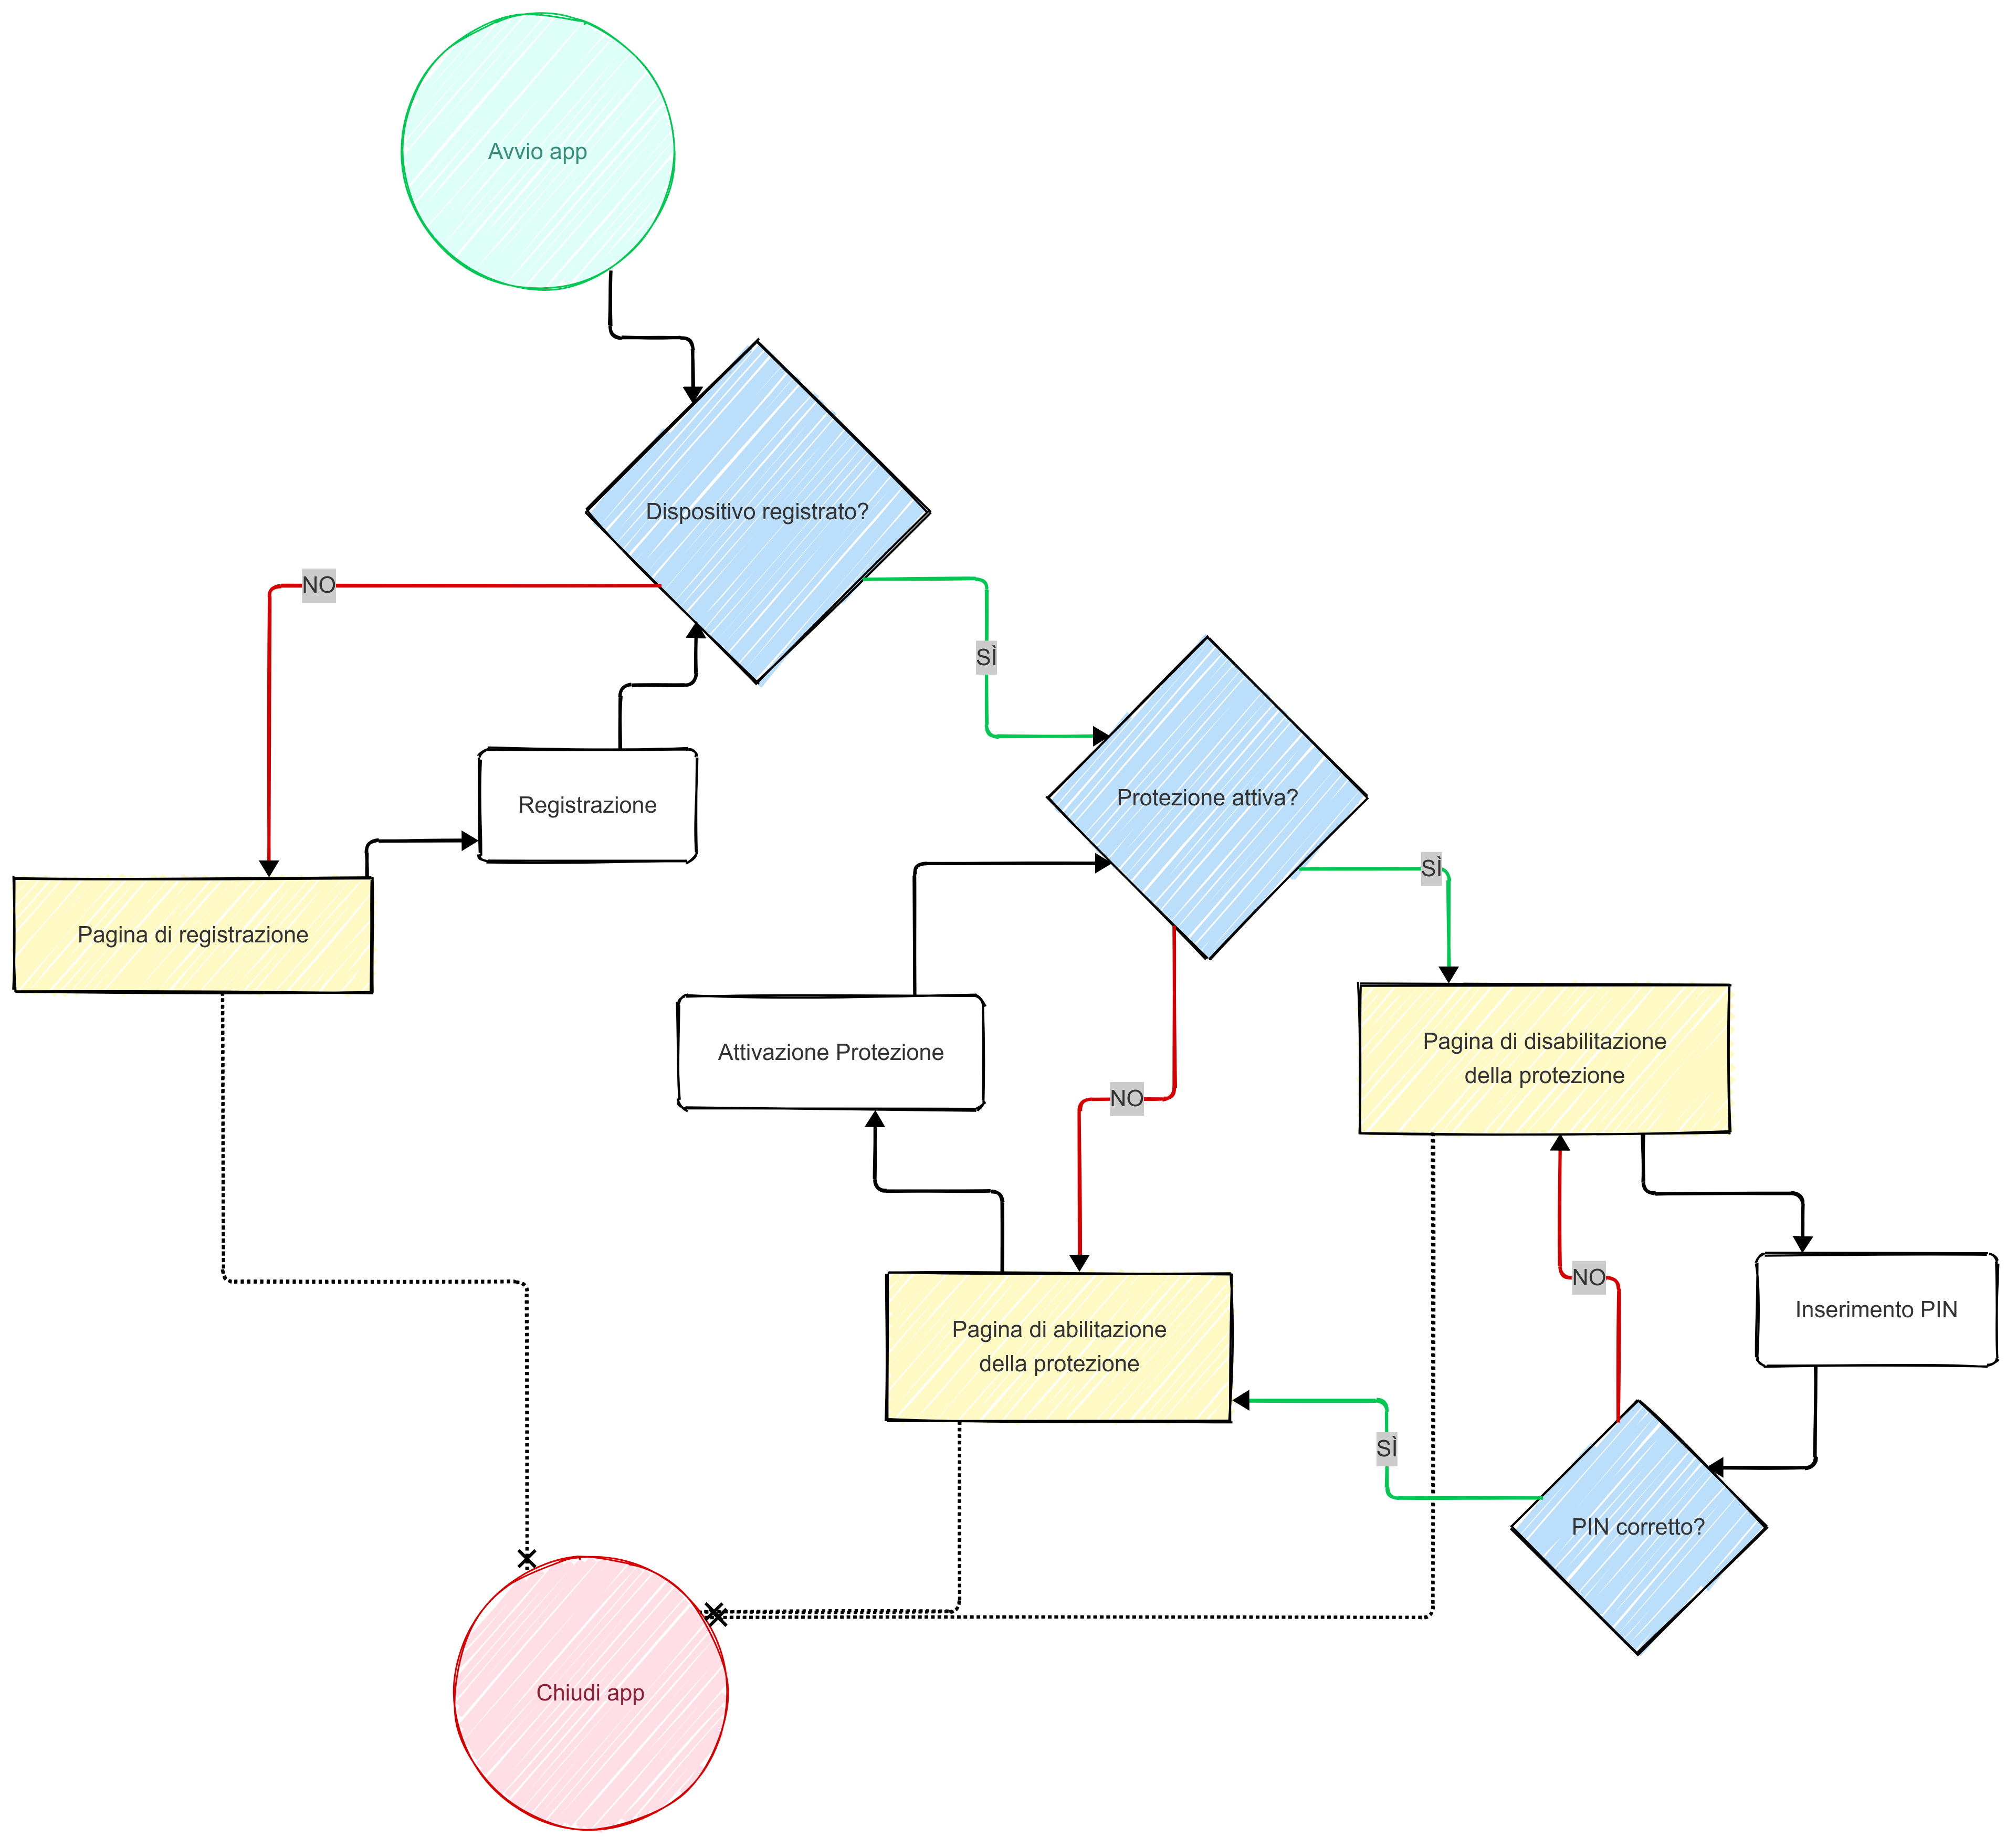
\includegraphics[width=1.0\textwidth]{figures/schema-casi-uso.png}
	\caption{navigazione dell'utente nell'app}
	\label{fig:schema-casi-uso}
\end{figure}

%---------------------------------------------------
% CAPITOLO 3
%---------------------------------------------------

\chapter{Analisi e progettazione}
\label{chap:analisi-e-progettazione}

\section{Struttura del progetto}

Lo sviluppo del progetto è stato naturalmente preceduto da una necessaria fase di analisi.
Identificati i requisiti del sistema, espressi nel capitolo \ref{chap:analisi-dei-requisiti}, risulta necessario definire come debba essere strutturato il software sulla base di essi.
Durante l'intera fase di progettazione si è tenuto conto del fatto che ClientShield ha come target di piattaforma Windows, in particolare a partire dalla versione 10.

Dall'analisi dei requisiti emerge chiaramente la presenza di due componenti ben distinti.
ClientShield, infatti, dovrà costantemente filtrare richieste \gls{DNS}, interagendo in maniera continuativa con il sistema operativo.
L'interazione diretta con l'utente, invece, è sporadica e avviene soltanto in caso di necessità, attraverso un'interfaccia grafica.
Per tale motivo, si è deciso fin da subito di suddividere lo sviluppo del software in due sotto-progetti, collegati tra loro, ma ben distinti.
Un'organizzazione di questo tipo permette di ottenere vantaggi importanti.

Anzitutto, la divisione in due sotto-progetti induce ad una minore complessità generale del sistema e ad una chiara suddivisione delle responsabilità.
Tale approccio, inoltre, da un punto di vista aziendale, facilita la gestione del codice e un'eventuale suddivisione del lavoro tra più sviluppatori.

In secondo luogo, sebbene il servizio di filtraggio debba necessariamente interagire con il sistema operativo, l'interfaccia utente e la logica di configurazione del filtro non hanno vincoli di piattaforma.
Ciò apre la possibilità ad una potenziale estensione multi-platform\footnote{La programmazione \textbf{multi-platform} si pone l'obiettivo di consentire allo stesso codice di poter essere eseguito su macchine aventi sistemi operativi differenti.} per la parte grafica.
Di conseguenza, un'eventuale espansione a sistemi operativi diversi (ad esempio Linux) richiederebbe unicamente la modifica del modulo di filtraggio.

\subsection{Organizzazione dei sotto-progetti}
\label{ssec:organizzazione-sotto-progetti}

Sulla base di questa suddivisione logica, ClientShield è stato organizzato in quattro diversi sotto-progetti:

\begin{itemize}
	\item \textbf{Servizio di filtraggio:}
	questo modulo rappresenta la parte centrale del software, sarà il responsabile dell'intercettazione e del filtraggio delle richieste \gls{DNS}.
	Dovrà essere implementato come servizio Windows, garantendo un'esecuzione continua e automatica all'avvio del sistema, definendo inoltre strategie di recupero in caso di errori.
	
	\item \textbf{Interfaccia utente:}
	questo modulo rappresenta la parte del software con cui l'utente interagirà.
	Il ruolo del sotto-progetto è di consentire la comunicazione con il servizio di filtraggio attraverso un'interfaccia grafica intuitiva.
	
	\item \textbf{Modulo comune:}
	questo modulo conterrà variabili, classi e configurazioni condivise tra interfaccia e servizio di filtraggio.
	Qui saranno specificati anche i tipi di messaggio che possono essere scambiati tra servizio e interfaccia, permettendo di mantenere sempre integrità di comunicazione tra i due sotto-progetti.
	
	\item \textbf{Installer:}
	questo modulo è dedicato alla creazione dell'installer del software.
	Si occuperà di automatizzare l'installazione del servizio e dell'interfaccia, garantendone il funzionamento corretto.
\end{itemize}
L'organizzazione della directory del progetto finale seguirà il più possibile la struttura illustrata in figura \ref{fig:struttura-directory-clientshield}.

\begin{figure}[H]
	\centering
	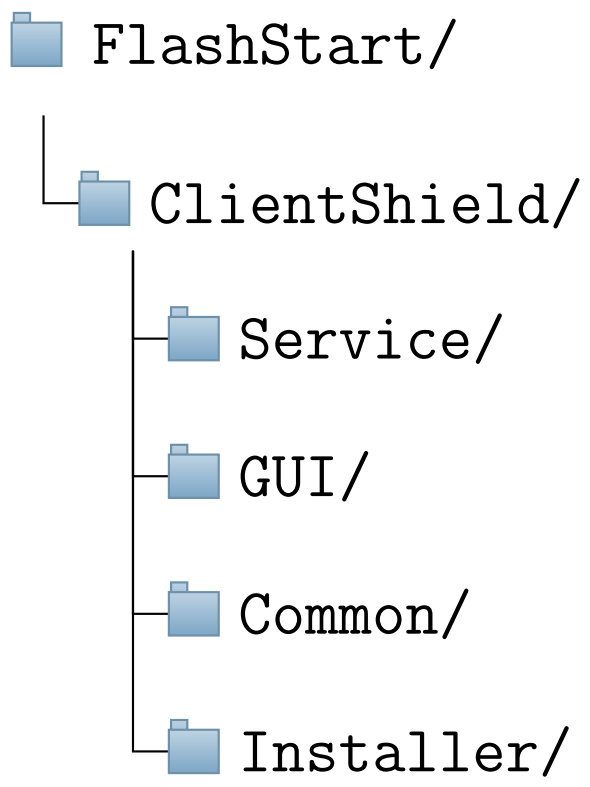
\includegraphics[width=0.3\textwidth]{figures/directory.png}
	\caption{Struttura dei sotto-progetti di ClientShield}
	\label{fig:struttura-directory-clientshield}
\end{figure}

\section{Comunicazione interprocesso}

Vista la divisione in progetti separati, la successiva fase di analisi ha preso in considerazione la modalità di comunicazione tra i due progetti.
L'architettura generale di ClientShield assomiglia molto ad un sistema client-server.
Infatti, l'interfaccia grafica deve stabilire una connessione con il servizio Windows per inviare dei messaggi contenenti gli input dell'utente e la richiesta di svolgere determinate operazioni, per poi attendere la risposta del servizio.

Per permettere la corretta comunicazione tra il servizio Windows e l'interfaccia grafica, è necessario stabilire un protocollo di comunicazione inter-processo.
Le caratteristiche fondamentali di tale protocollo sono garantire una comunicazione affidabile e di tipo half-duplex\footnote{La comunicazione \textbf{half-duplex} tra due nodi permette la trasmissione di messaggi da parte di entrambi, ma soltanto uno per volta.} tra due processi separati, ma in esecuzione sullo stesso dispositivo.

Per la scelta del protocollo, dovendo sviluppare in ambiente Windows, ci si è riferiti alla documentazione Microsoft, che presenta l'articolo \cite{MicrosoftIPC2024} sulle comunicazioni inter-processo.
Si è optato per l'utilizzo della comunicazione tramite named pipes, consigliata soprattutto per la sua affidabilità e semplicità di implementazione, grazie al supporto nativo offerto da Windows.

Le named pipes permettono di stabilire un canale di comunicazione identificato da un nome univoco, accessibile sia dal servizio che dall'interfaccia senza necessità di configurazioni complesse.   
Un ulteriore vantaggio è la loro efficienza: essendo ottimizzate per la comunicazione all'interno dello stesso sistema, garantiscono una latenza ridotta rispetto ad altre tecniche di comunicazione inter-processo.  
Infine le named pipes offrono la possibilità di definire controlli di accesso a livello di sistema operativo, impedendo la manipolazione dei dati da parte di processi non autorizzati, garantendo che solo l'interfaccia ufficiale possa inviare comandi al servizio, evitando interferenze da applicazioni di terze parti.

Scelto il protocollo, si è scelta la struttura dei messaggi.
Vista la vasta disponibilità di librerie capaci di serializzare e deserializzare classi in formato JSON, si è deciso di utilizzare quest'ultimo per la comunicazione.
La scelta è dovuta al fatto che i dati presenti nel messaggio dipendono dall'operazione e possono essere anche di tipo diverso. Infatti la disabilitazione, come sottolineato in sezione \ref{sec:casi-d-uso}, necessita l'inserimento di un numero intero.
Ciò significa che l'invio di semplici stringhe di testo richiederebbe controlli manuali sulla struttura del messaggio e sui tipi di ogni singolo campo.
JSON permette l'automatizzazione dei controlli: sarà sufficiente definire delle classi rappresentanti i diversi tipi di messaggio nella comunicazione e delegare la conversione da classe a JSON, o viceversa, ad una libreria esterna, gestendo eventuali errori.

In figura \ref{fig:schema-messaggi-gui-service} viene illustrato il possibile scambio di messaggi tra interfaccia grafica e servizio Windows.

\begin{figure}[h]
	\centering
	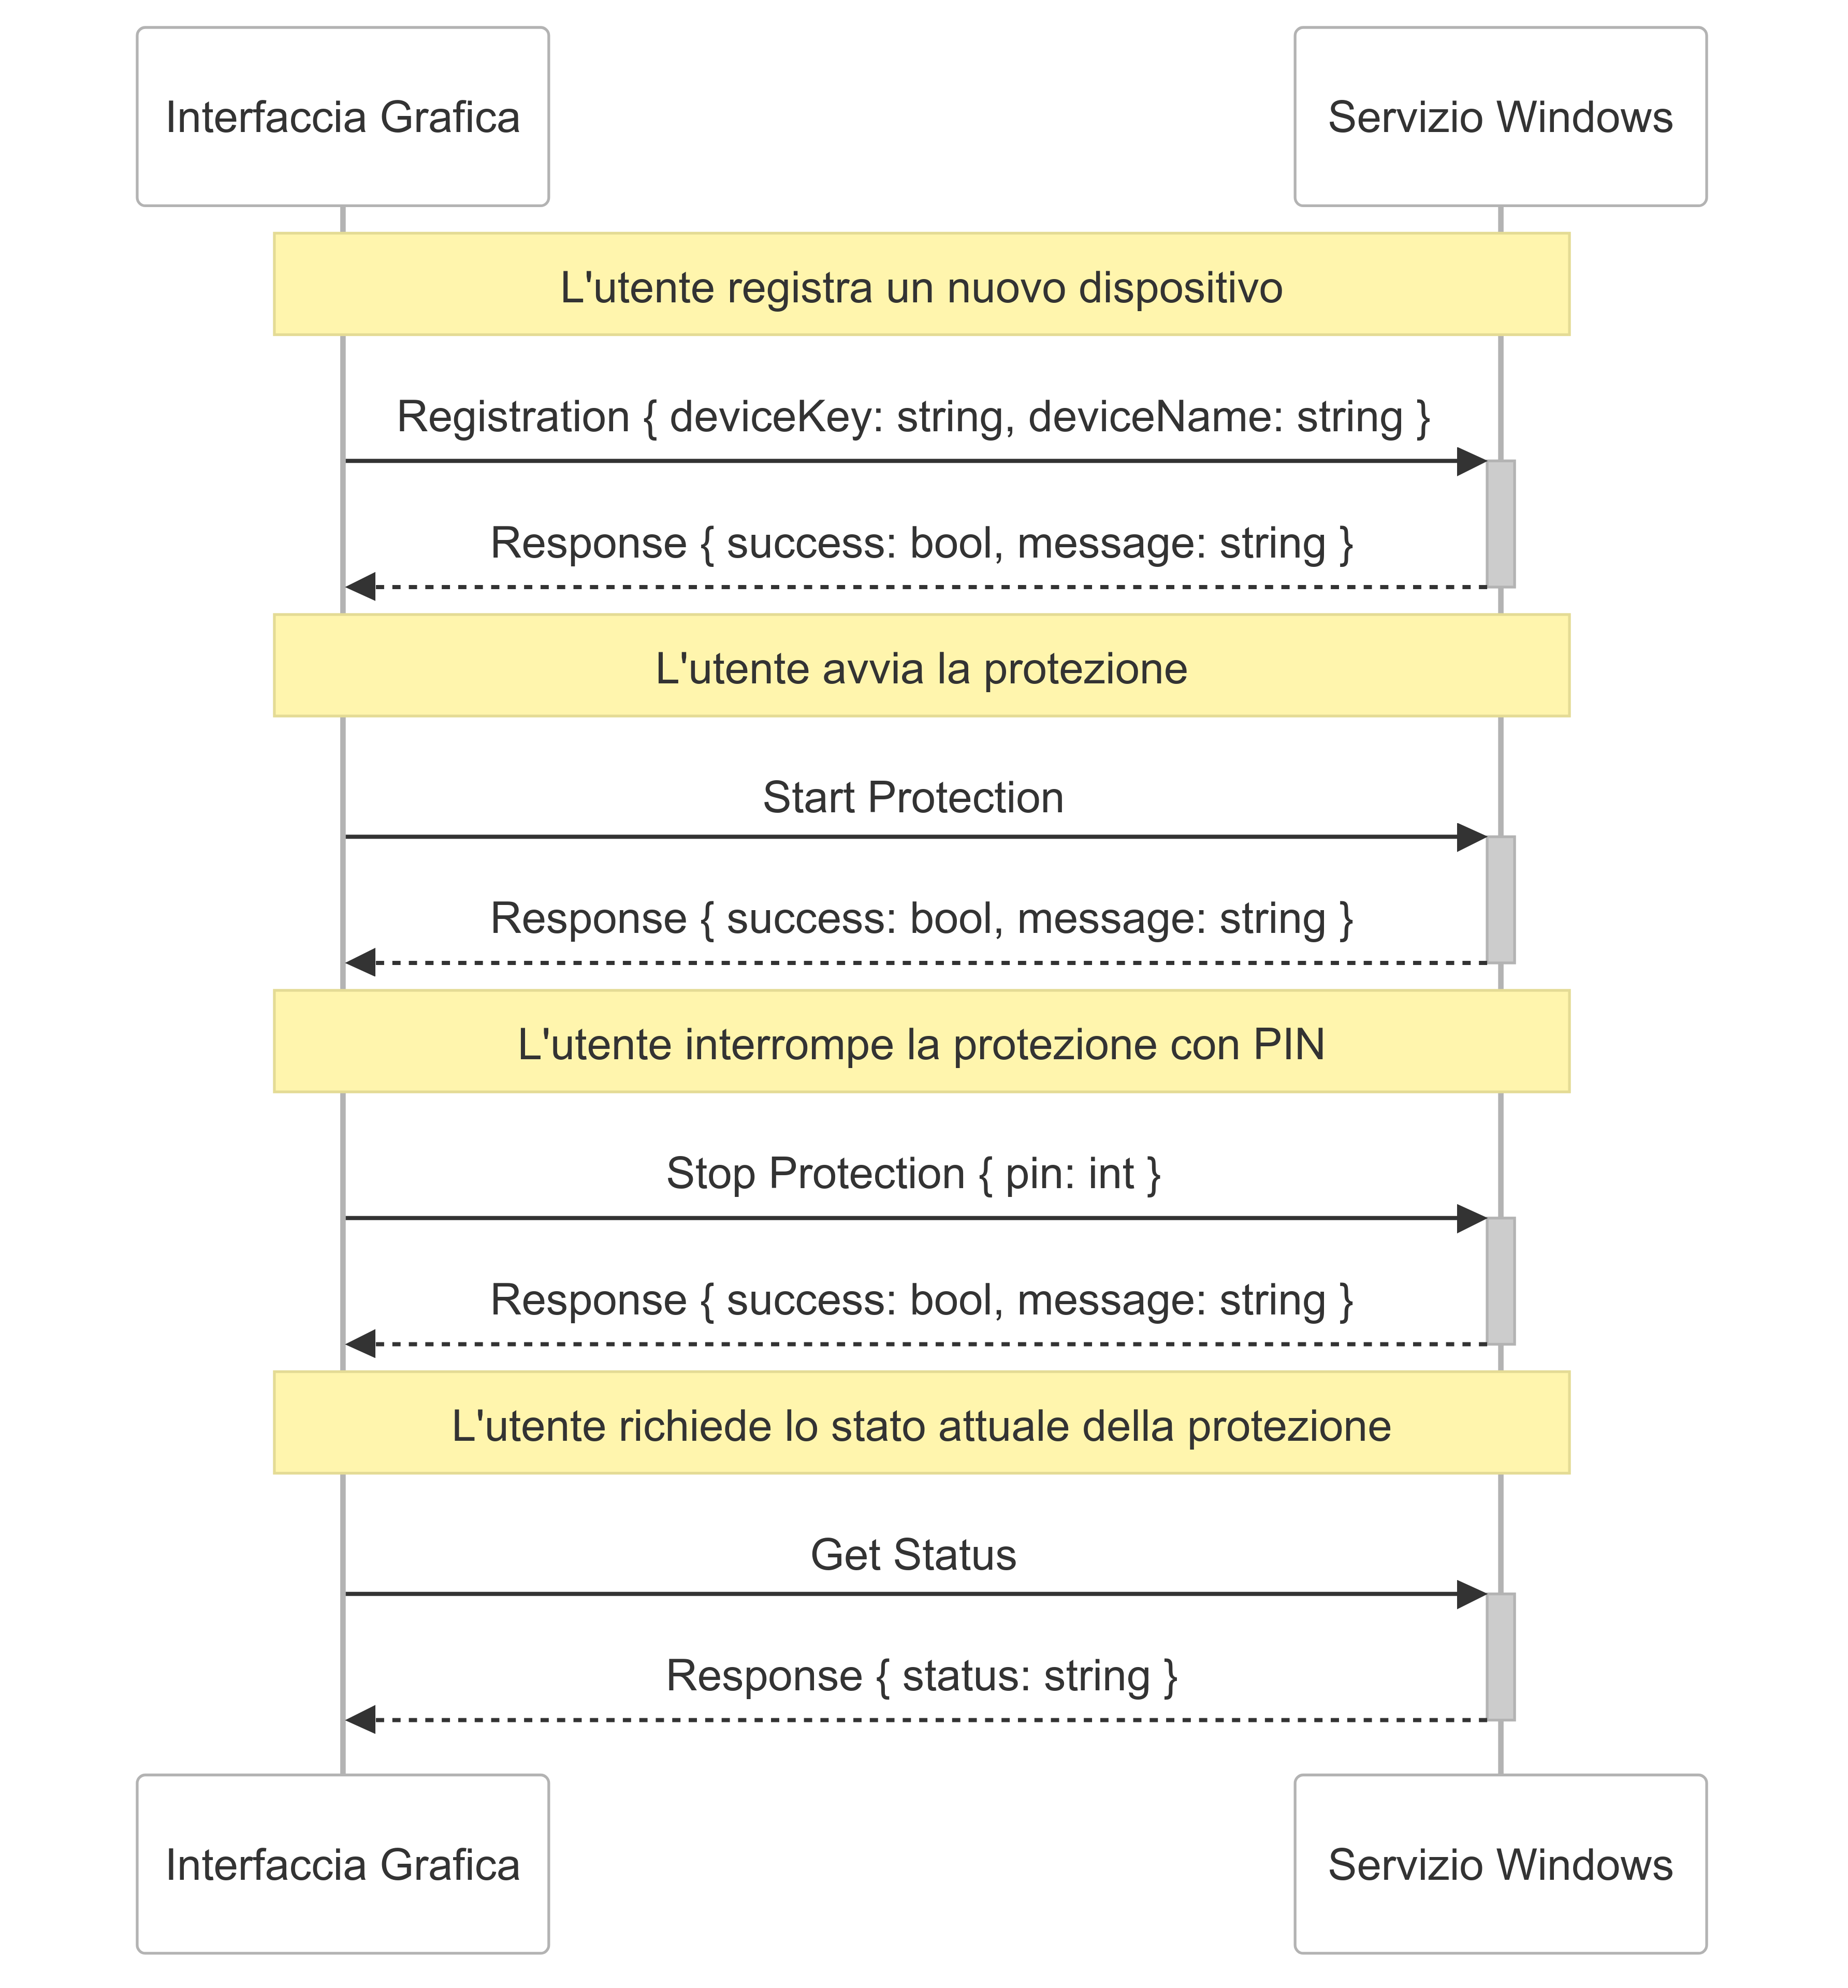
\includegraphics[width=0.7\textwidth]{figures/schema-messaggi-gui-service.png}
	\caption{Scambio di messaggi tra GUI e servizio Windows}
	\label{fig:schema-messaggi-gui-service}
\end{figure}

\section{Servizio Windows}

Il servizio di filtraggio si compone essenzialmente di due parti: una gestisce la comunicazione inter-processo, l'altra si occupa del filtraggio \gls{DNS}.
Dei due componenti, la comunicazione inter-processo deve essere sempre disponibile, ma il servizio di filtraggio si potrà attivare e disattivare a comando.
Per questo motivo, il servizio Windows deve essere costituito principalmente come un server named pipe, mentre l'analisi si concentra sull'organizzazione del servizio di protezione.

Nel vecchio software, per assicurare che tutto il traffico passasse dal filtro, veniva creata una scheda di rete virtuale.
Modificando le metriche di priorità delle interfacce si rendeva quest’ultima la più “alta in graduatoria”, così che il sistema instradasse il traffico su di essa prima di qualsiasi altra. Questo permetteva di intercettare le richieste e bloccare o modificare il traffico indesiderato. Tuttavia, si trattava di una soluzione più complessa da gestire e potenzialmente soggetta a conflitti con altri driver o componenti di rete.

Nella nuova versione di ClientShield, invece, si è deciso di implementare un server \gls{DNS} locale, soluzione che offre dei vantaggi considerevoli:

\begin{itemize}
	\item \textbf{Semplicità di implementazione:}
	configurare un processo che ascolti sulla porta 53 e risolva le richieste \gls{DNS} è decisamente più semplice rispetto alla creazione di una scheda di rete virtuale.
	Tale scelta, inoltre, limita anche il rischio di incompatibilità con software terzi che gestiscono altre schede di rete virtuali.
	
	\item \textbf{Manutenibilità:}
	un server locale consente di isolare la responsabilità del software semplicemente al filtraggio.
	Questa soluzione permette una maggiore chiarezza e una più corretta aderenza al \gls{SRP}. %, descritto in \cite{Martin2002}.
	In questo modo, infatti, il modulo di protezione gestisce solo richieste \gls{DNS}, migliorando il debugging, che sarà limitato ad un singolo componente.
	
	\item \textbf{Portabilità:}
	l'implementazione di un server \gls{DNS} non ha dipendenze specifiche dal sistema operativo.
	Le soluzioni esplorate in seguito consentono di relegare l'interazione diretta con il sistema operativo alla sola impostazione del server locale come \gls{DNS} predefinito.
\end{itemize}

In sintesi, il nuovo design del servizio Windows prevede l'implementazione di un server named pipe che, su comando dell'utente, interagisca con il servizio di protezione per avviare l'esecuzione di un server \gls{DNS} locale, impostandolo come predefinito di sistema, oppure interromperla.

Tutti i pattern utilizzati nella progettazione del servizio Windows (sezioni \ref{ssec:analisi-protezione} e \ref{ssec:analisi-server-dns}) fanno riferimento al libro \cite{GoF94}.

\subsection{Analisi della protezione}
\label{ssec:analisi-protezione}

L'avvio della protezione è un problema più complesso di quanto possa sembrare.
Per attivarla è necessaria l'interazione con molti componenti del sistema.
Il server named pipe dovrebbe gestire le API FlashStart, occupandosi della registrazione, dell'autorizzazione e dei controlli periodici sullo stato del servizio.
Inoltre, deve monitorare lo stato del server \gls{DNS} e interagire con esso, permettendone il riavvio e l'arresto automatici o su richiesta. 
In aggiunta, il servizio deve occuparsi anche della gestione delle credenziali, memorizzando il codice utente fornito durante la registrazione e garantendo il ripristino della sessione al riavvio del dispositivo.

Per una corretta delegazione delle responsabilità e per ottenere semplicità nella comunicazione con diversi componenti, è stato sfruttato il pattern \textit{Facade}.
Questo pattern fornisce una semplice interfaccia che consente la gestione di funzionalità distribuite su più classi.

Dalla struttura delle classi, illustrata in figura \ref{fig:protezione-facade-pattern}, è possibile constatare che la classe \texttt{ServerNamedPipe} si occupa esclusivamente di ricevere ed elaborare le richieste da parte del client, delegando l'esecuzione di qualsiasi operazione alla classe \texttt{ProtectionManager}.
Quest'ultima funge da punto di raccordo tra le diverse funzionalità offerte dal software, gestendole in maniera organizzata, permettendo una granularità maggiore che facilita la manutenzione del codice.
\begin{figure}[h]
	\centering
	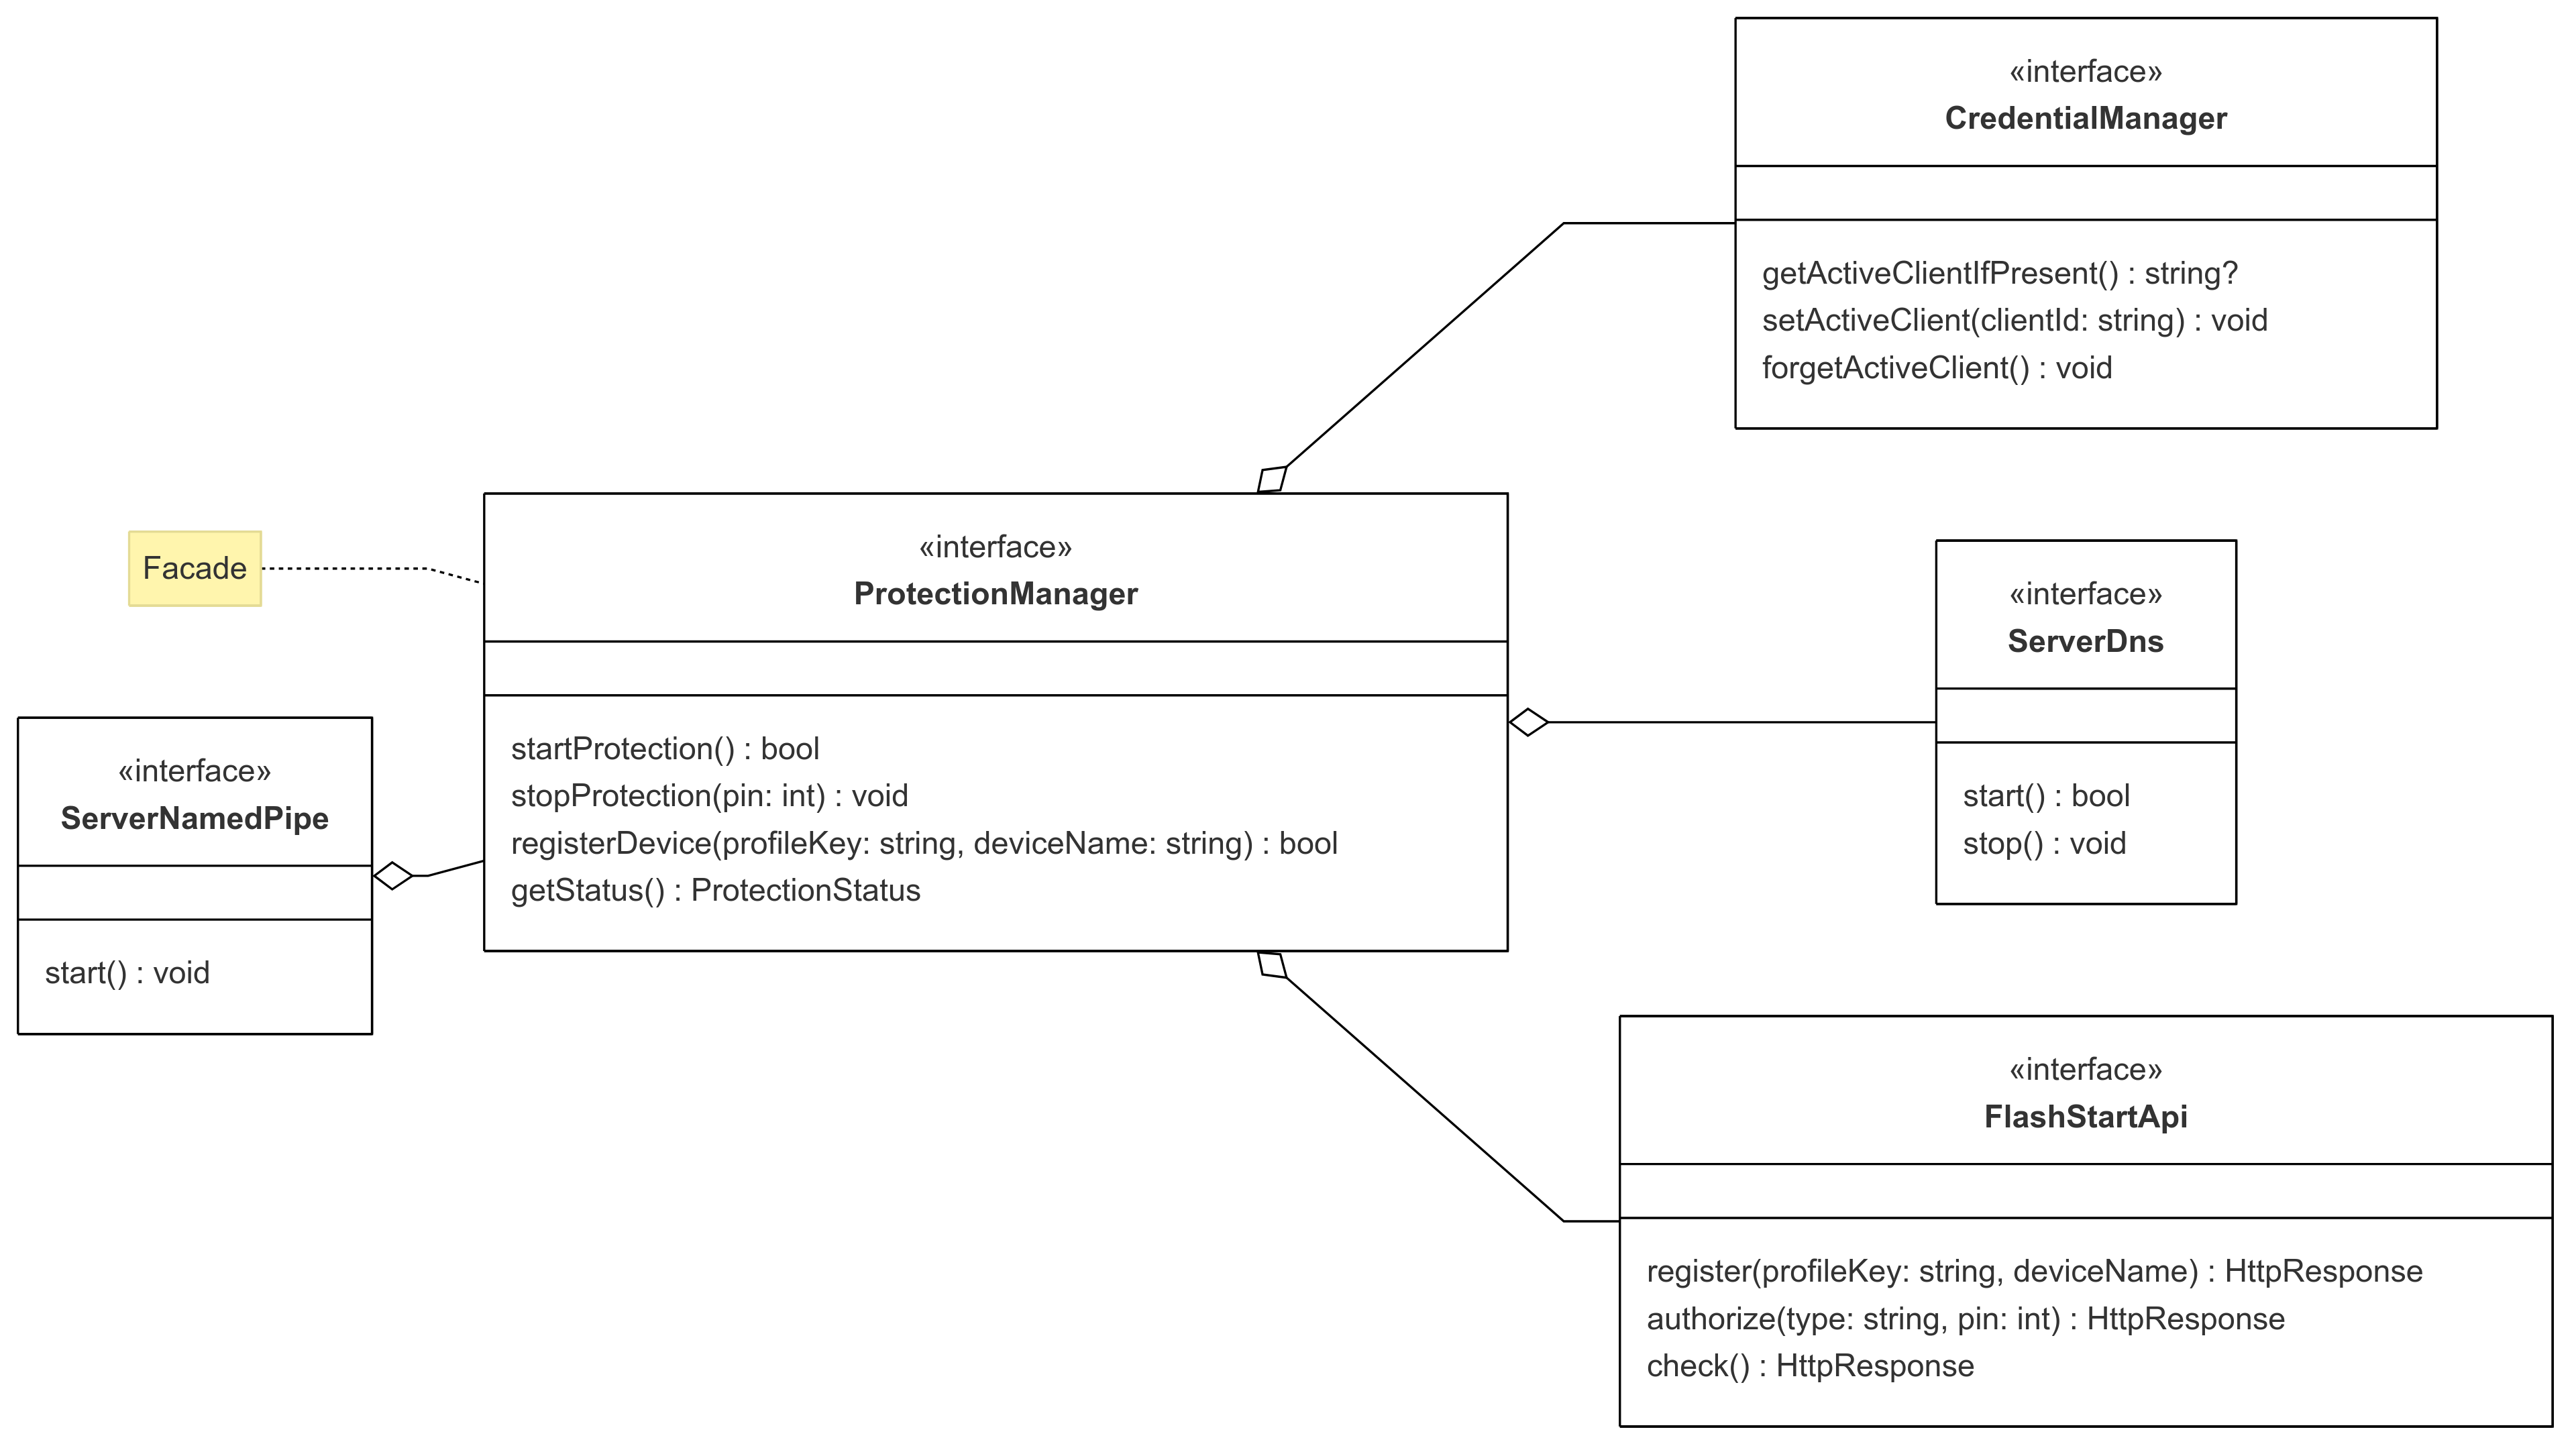
\includegraphics[width=1.0\textwidth]{figures/protezione-facade-pattern.png}
	\caption{Facade pattern per la gestione della protezione}
	\label{fig:protezione-facade-pattern}
\end{figure}
\texttt{ProtectionManager} coordina l'esecuzione delle funzionalità offerte dalle classi gestite, consentendo una gestione implicita delle credenziali affidata completamente a \texttt{CredentialManager}.
Inoltre, \texttt{ProtectionManager} verifica costantemente la coerenza tra lo stato dei componenti e, se presente una sessione attiva, avvia automaticamente la protezione.


\subsection{Analisi server DNS}
\label{ssec:analisi-server-dns}

Il server \gls{DNS} locale rappresenta il nucleo centrale di ClientShield, poiché gestisce sia la risoluzione dei domini che l'applicazione dei filtri.
Per garantire flessibilità ed estensibilità, il server è stato suddiviso in più componenti, ciascuno con una funzionalità specifica.
La scelta è motivata da due fattori principali.
In primo luogo, suddividere il server in componenti più piccoli ne facilita l'estensibilità, consentendo di aggiungere nuove funzioni senza alterare la struttura di base.
Inoltre, la suddivisione delle funzionalità consente il più facile impiego di thread-pools, consentendo la creazione di worker sulla base dei componenti.

\begin{figure}[H]
	\centering
	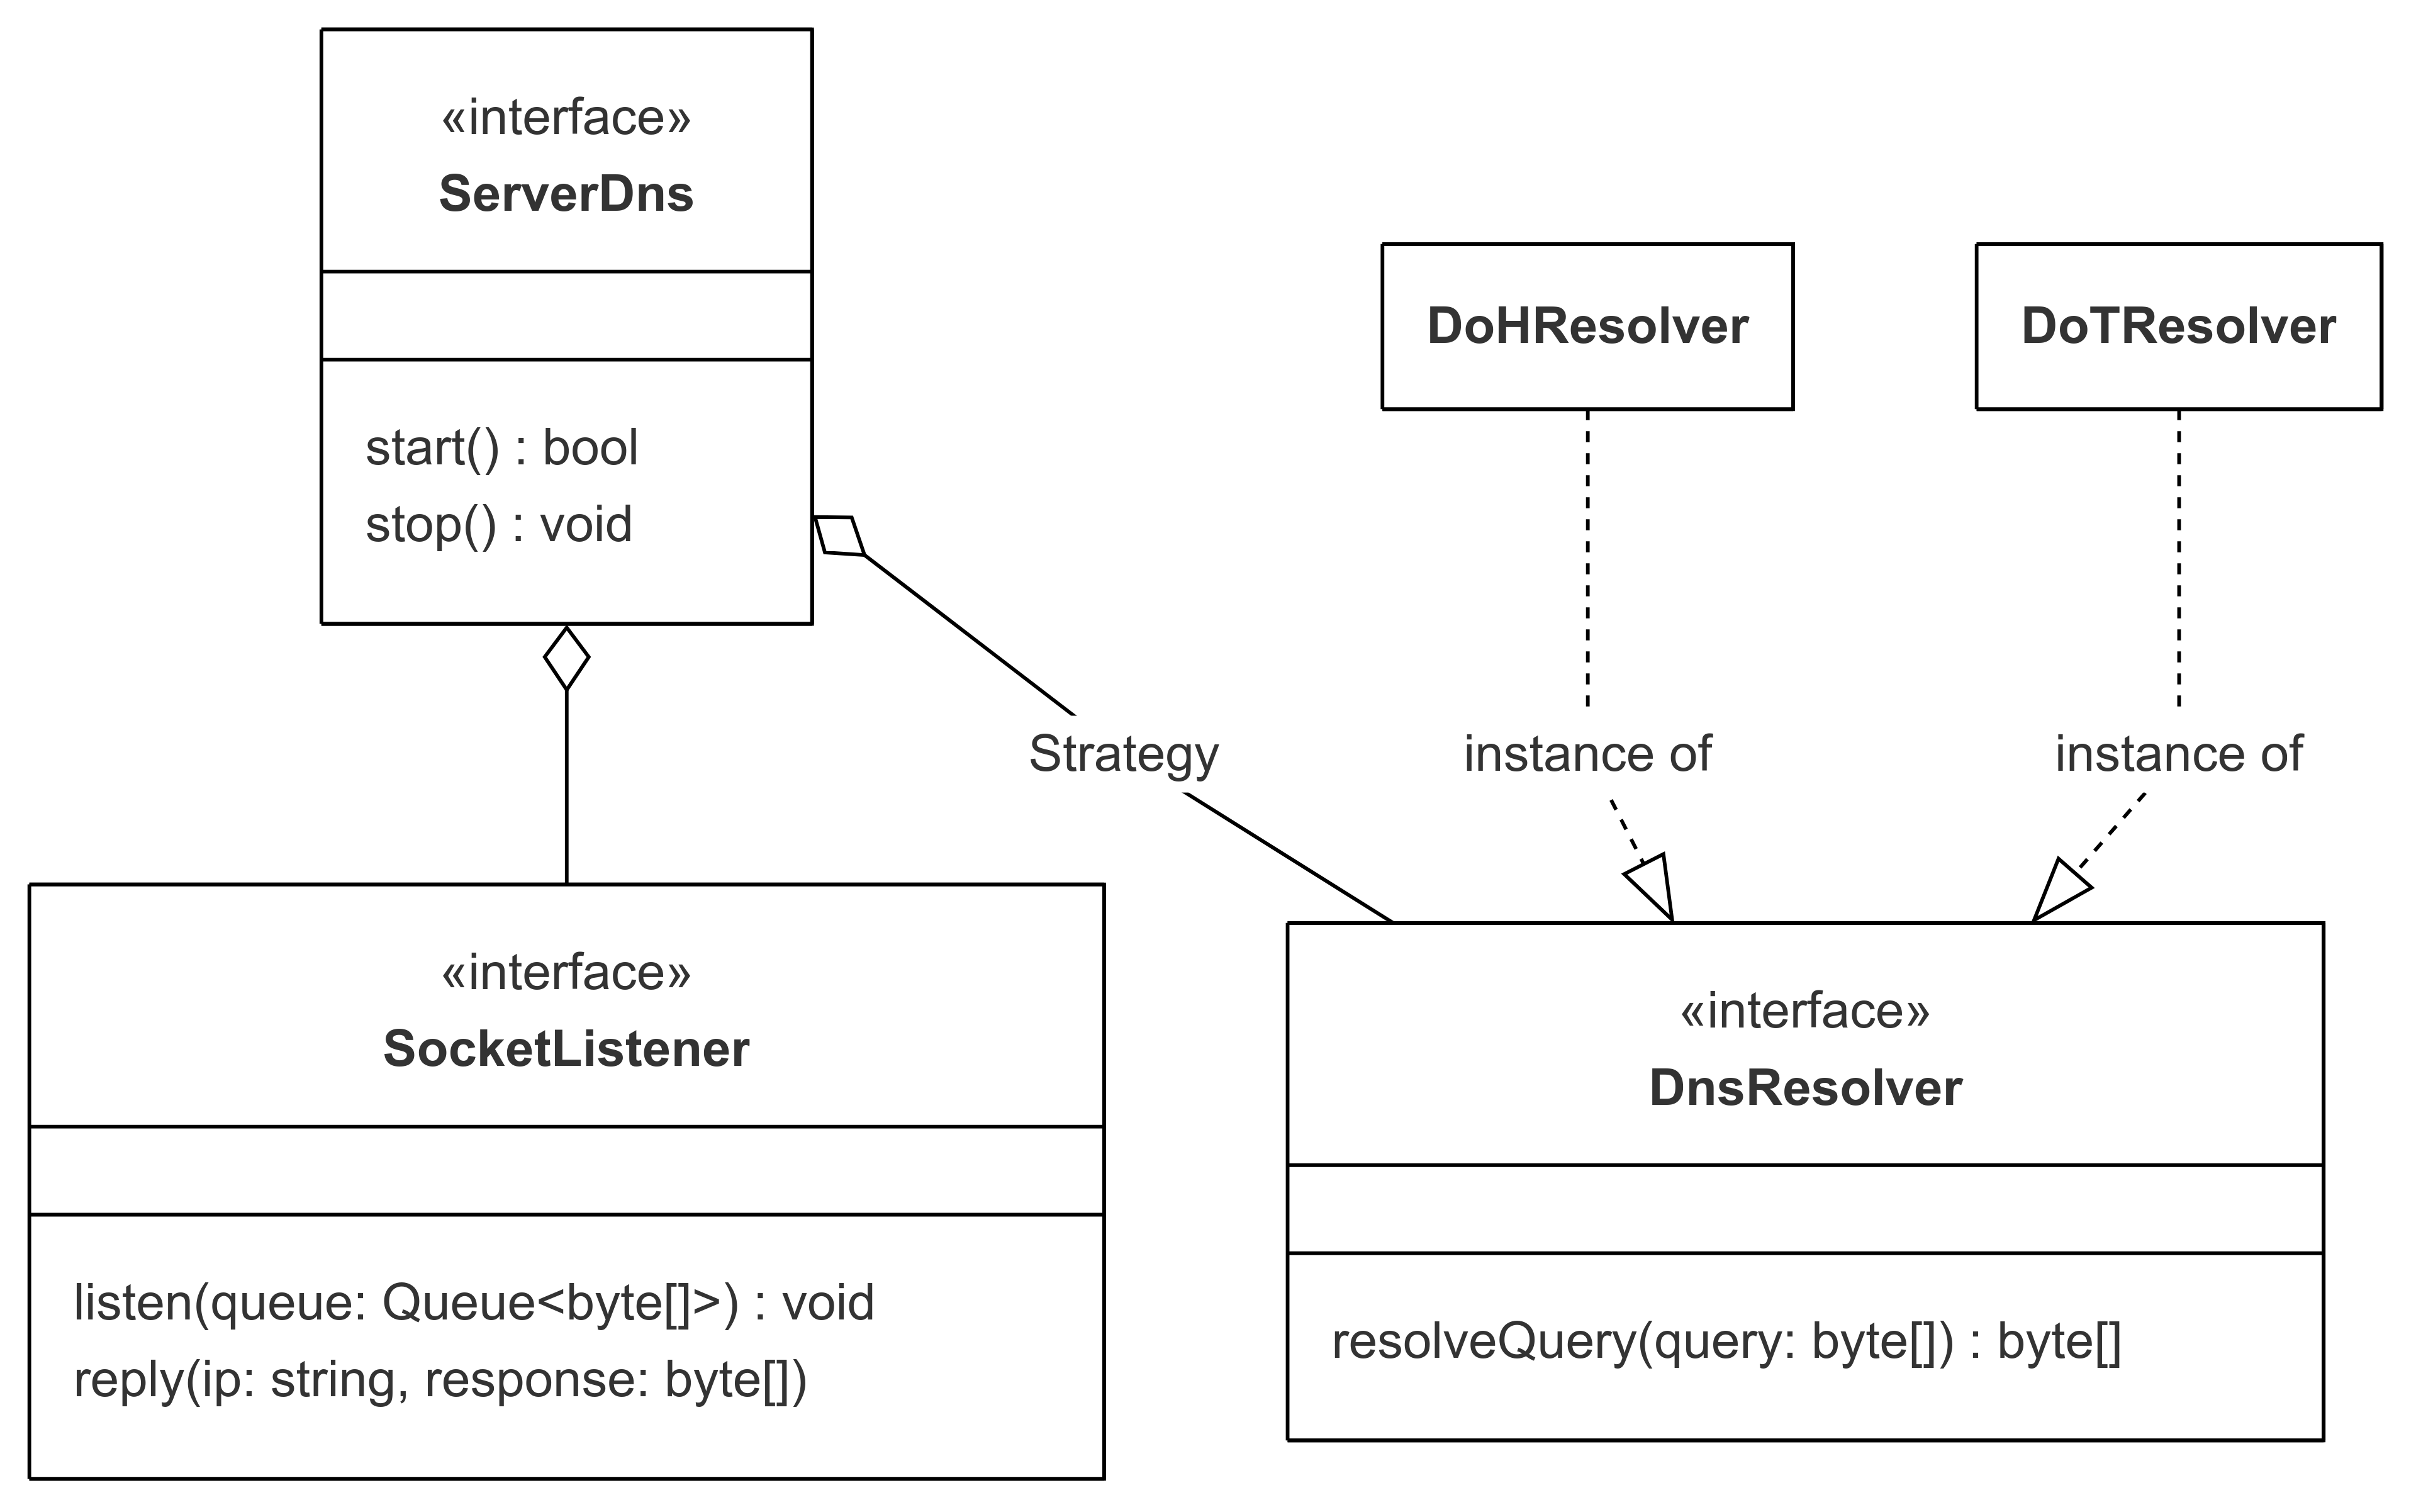
\includegraphics[width=0.8\textwidth]{figures/dns-strategy-pattern.png}
	\caption{Strategy pattern per Server DNS}
	\label{fig:dns-strategy-pattern}
\end{figure}
Come illustrato in figura \ref{fig:dns-strategy-pattern}, \texttt{DnsServer} utilizza il pattern \textit{Strategy} per la risoluzione dei domini.
Delegando la risoluzione dei domini a una classe secondaria, \texttt{DnsResolver}, è possibile implementare tecnologie differenti.
Sebbene i requisiti del prototipo richiedano la sola implementazione \gls{DoH}, FlashStart ha già implementato delle API che utilizzano il protocollo \gls{DoT}.
Se in futuro l'azienda decidesse di adottare \gls{DoT} o un qualsiasi altro tipo di tecnologia per la risoluzione dei domini, sarà sufficiente sostituire il \texttt{DnsResolver} con un'implementazione specifica, senza modificare il resto del sistema.


Un altro aspetto fondamentale riguarda la gestione delle richieste in ingresso.  
Poiché la porta 53, dedicata alla comunicazione \gls{DNS}, può essere gestita da un solo componente alla volta, la ricezione dei pacchetti è affidata alla classe \texttt{SocketListener}. 
Tale entità ha il compito di minimizzare i tempi di gestione delle query in arrivo, prevenendo la perdita di richieste.
Per massimizzare l'efficienza, \texttt{SocketListener} utilizzerà una coda di messaggi, permettendo alla classe \texttt{DnsServer} di elaborare le richieste in parallelo.
Se necessario, potranno essere utilizzati worker dedicati per ottimizzare le prestazioni e garantire l'elevata reattività del sistema.

\begin{figure}[H]
	\centering
	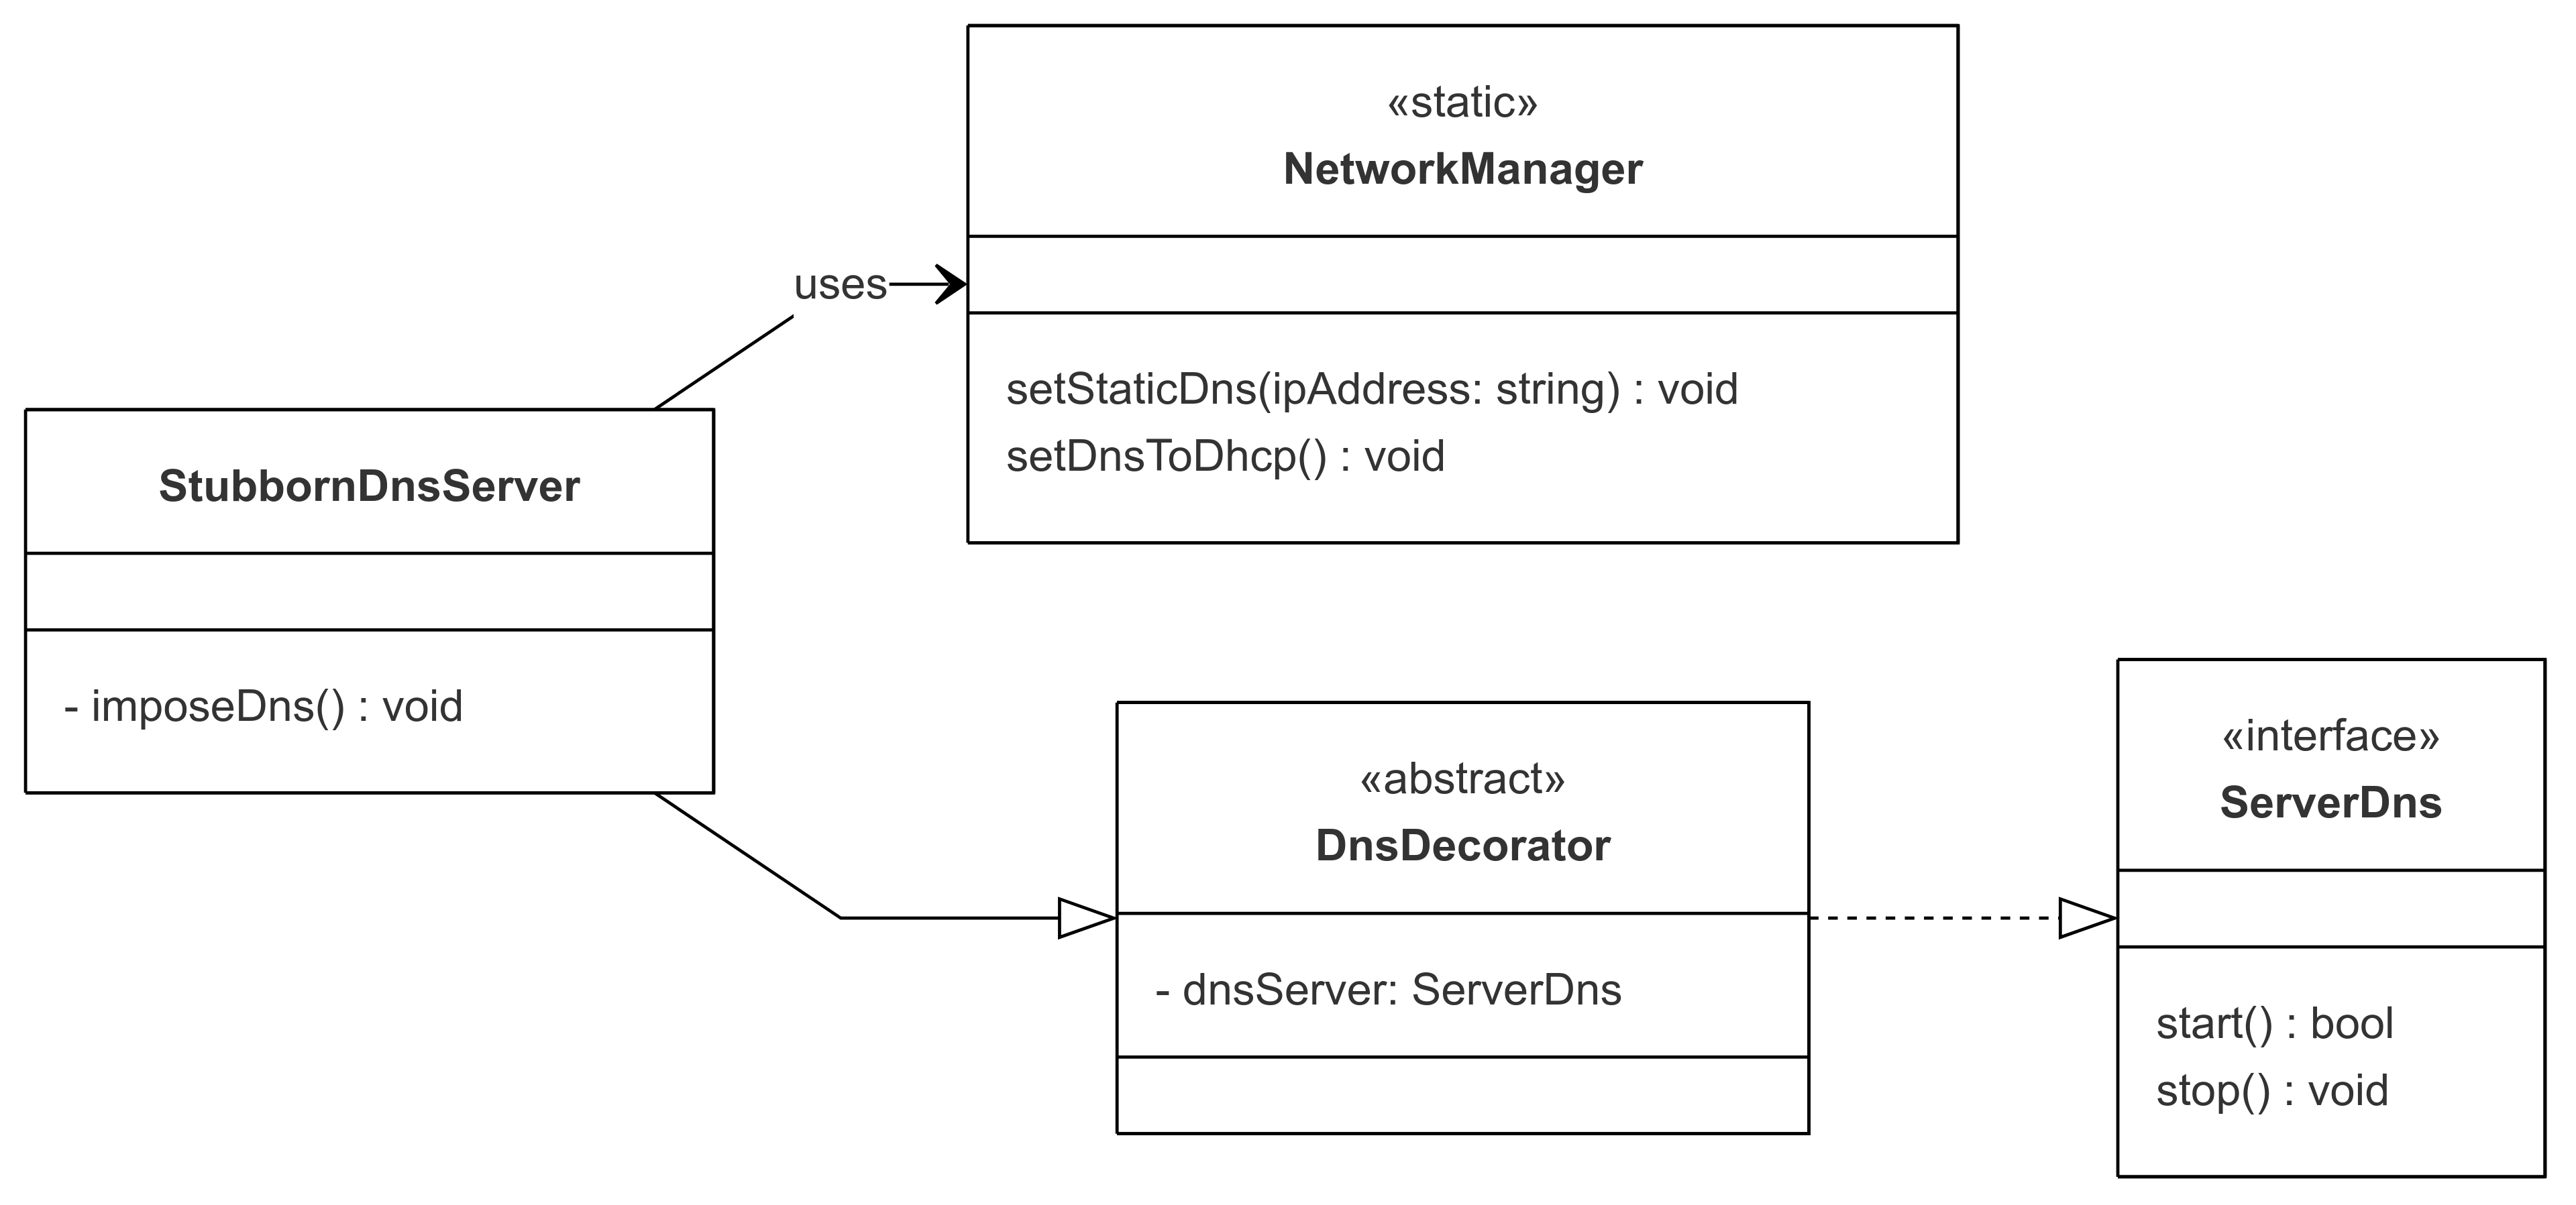
\includegraphics[width=0.8\textwidth]{figures/dns-decorator-pattern.png}
	\caption{Decorator pattern per Server DNS}
	\label{fig:dns-decorator-pattern}
\end{figure}
Infine, l'ultimo e cruciale compito affidato al servizio Windows è impostare il server \gls{DNS} locale come predefinito di sistema.
Questa fase è decisamente delicata, perché rappresenta il punto in cui ClientShield interagisce direttamente con il sistema operativo, diventando di fatto dipendente dalla piattaforma.

La soluzione utilizzata in questo caso, illustrata in figura \ref{fig:dns-decorator-pattern}, sfrutta il pattern \textit{Decorator}.
Questa scelta permette di isolare la logica di interazione con Windows in una classe secondaria, migliorando il riuso.
Ad interagire con il sistema operativo è la classe statica \texttt{NetworkManager}, che consente di configurare il \gls{DNS} di sistema come statico, specificando un indirizzo, oppure di ripristinarlo in modalità dinamica.
Il decoratore \texttt{StubbornDnsServer} permette di aggiungere le funzionalità di \texttt{NetworkManager} a \texttt{DnsServer}.
In questo modo è possibile estendere i metodi per avviare e interrompere il server, garantendo, rispettivamente, l'aggiornamento e il ripristino automatico del \gls{DNS} predefinito sul dispositivo.
L'adozione del pattern \textit{Decorator} risulta particolarmente utile, in quanto consente di isolare l'utilizzo di librerie specifiche per Windows a due sole classi, aprendo la possibilità ad un futuro sviluppo multi-platform.

\section{Interfaccia grafica}

L'interfaccia grafica è l'unica parte del software con cui l'utente interagirà direttamente.
Il suo compito è essenzialmente quello di permettere all'utilizzatore l'accesso ai comandi della protezione, esposti tramite il server pipe dal servizio Windows.
L'interfaccia agisce come client nella connessione tramite named pipe, inviando le richieste effettuate dall'utente e attendendo la risposta dal server.

Poiché il software è soltanto un prototipo, l'obiettivo dell'analisi è proporre una soluzione che permetta una facile modifica della parte visiva.
L'interfaccia sarà sviluppata molto semplicemente, dando solo una rapida rappresentazione grafica ai comandi implementati.
Dal punto di vista aziendale, il prototipo risulta efficace se la modifica dell'interfaccia, che verrà senza dubbio sottoposta al consiglio di grafici esperti, richiede poche o nulle modifiche di backend.

\subsection{Model-View-Presenter}
\label{ssec:analisi-mvp}

Per lo sviluppo dell'interfaccia grafica è stato utilizzato il pattern architetturale \textit{\gls{MVP}}.
\gls{MVP} è un'architettura software che deriva dal famosissimo pattern \textit{\gls{MVC}}, nata con lo scopo di separare la logica di presentazione dall'interfaccia, in modo da migliorare la manutenibilità e il testing del codice.

Si compone di tre elementi principali:
\begin{itemize}
	\itemdef{Model:}
	offre un'interfaccia per reperire i dati che devono essere visualizzati, l'ottenimento dei quali può coinvolgere eventualmente anche la comunicazione tramite API.
	
	\itemdef{View:}
	è la parte responsabile della rappresentazione dei dati.
	La \textit{View} si occupa esclusivamente di eseguire chiamate al suo \textit{Presenter} ogni qual volta l'utente interagisca con l'interfaccia.
	Tipicamente è un componente totalmente passivo, le cui funzionalità sono ridotte al minimo e contengono poca, o nessuna logica.
	Non comunica direttamente con la parte di \textit{Model}, tutti i dati passano attraverso il \textit{Presenter}, lasciando alla \textit{View} il solo compito di rappresentarli visivamente.
	
	\itemdef{Presenter:} implementa l'intera logica di presentazione, occupandosi
	di reperire i dati dal \textit{Model} ed eventualmente modificarli in modo che
	possano essere rappresentati.
	Il \textit{Presenter}, inoltre, riceve i dati in input dalla \textit{View}, li valida e si occupa della loro elaborazione.
	Svolge il ruolo di mediatore tra \textit{Model} e \textit{View}, occupandosi di verificare sempre la coerenza tra dati e rappresentazione.
\end{itemize}
A causa della loro stretta interconnessione, Presenter e View detengono riferimenti reciproci, consentendo ad ognuno di chiamare i metodi dell'altro.
Ogni View necessita il suo specifico Presenter e tipicamente lo instanzia essa stessa.

\begin{figure}[H]
	\centering
	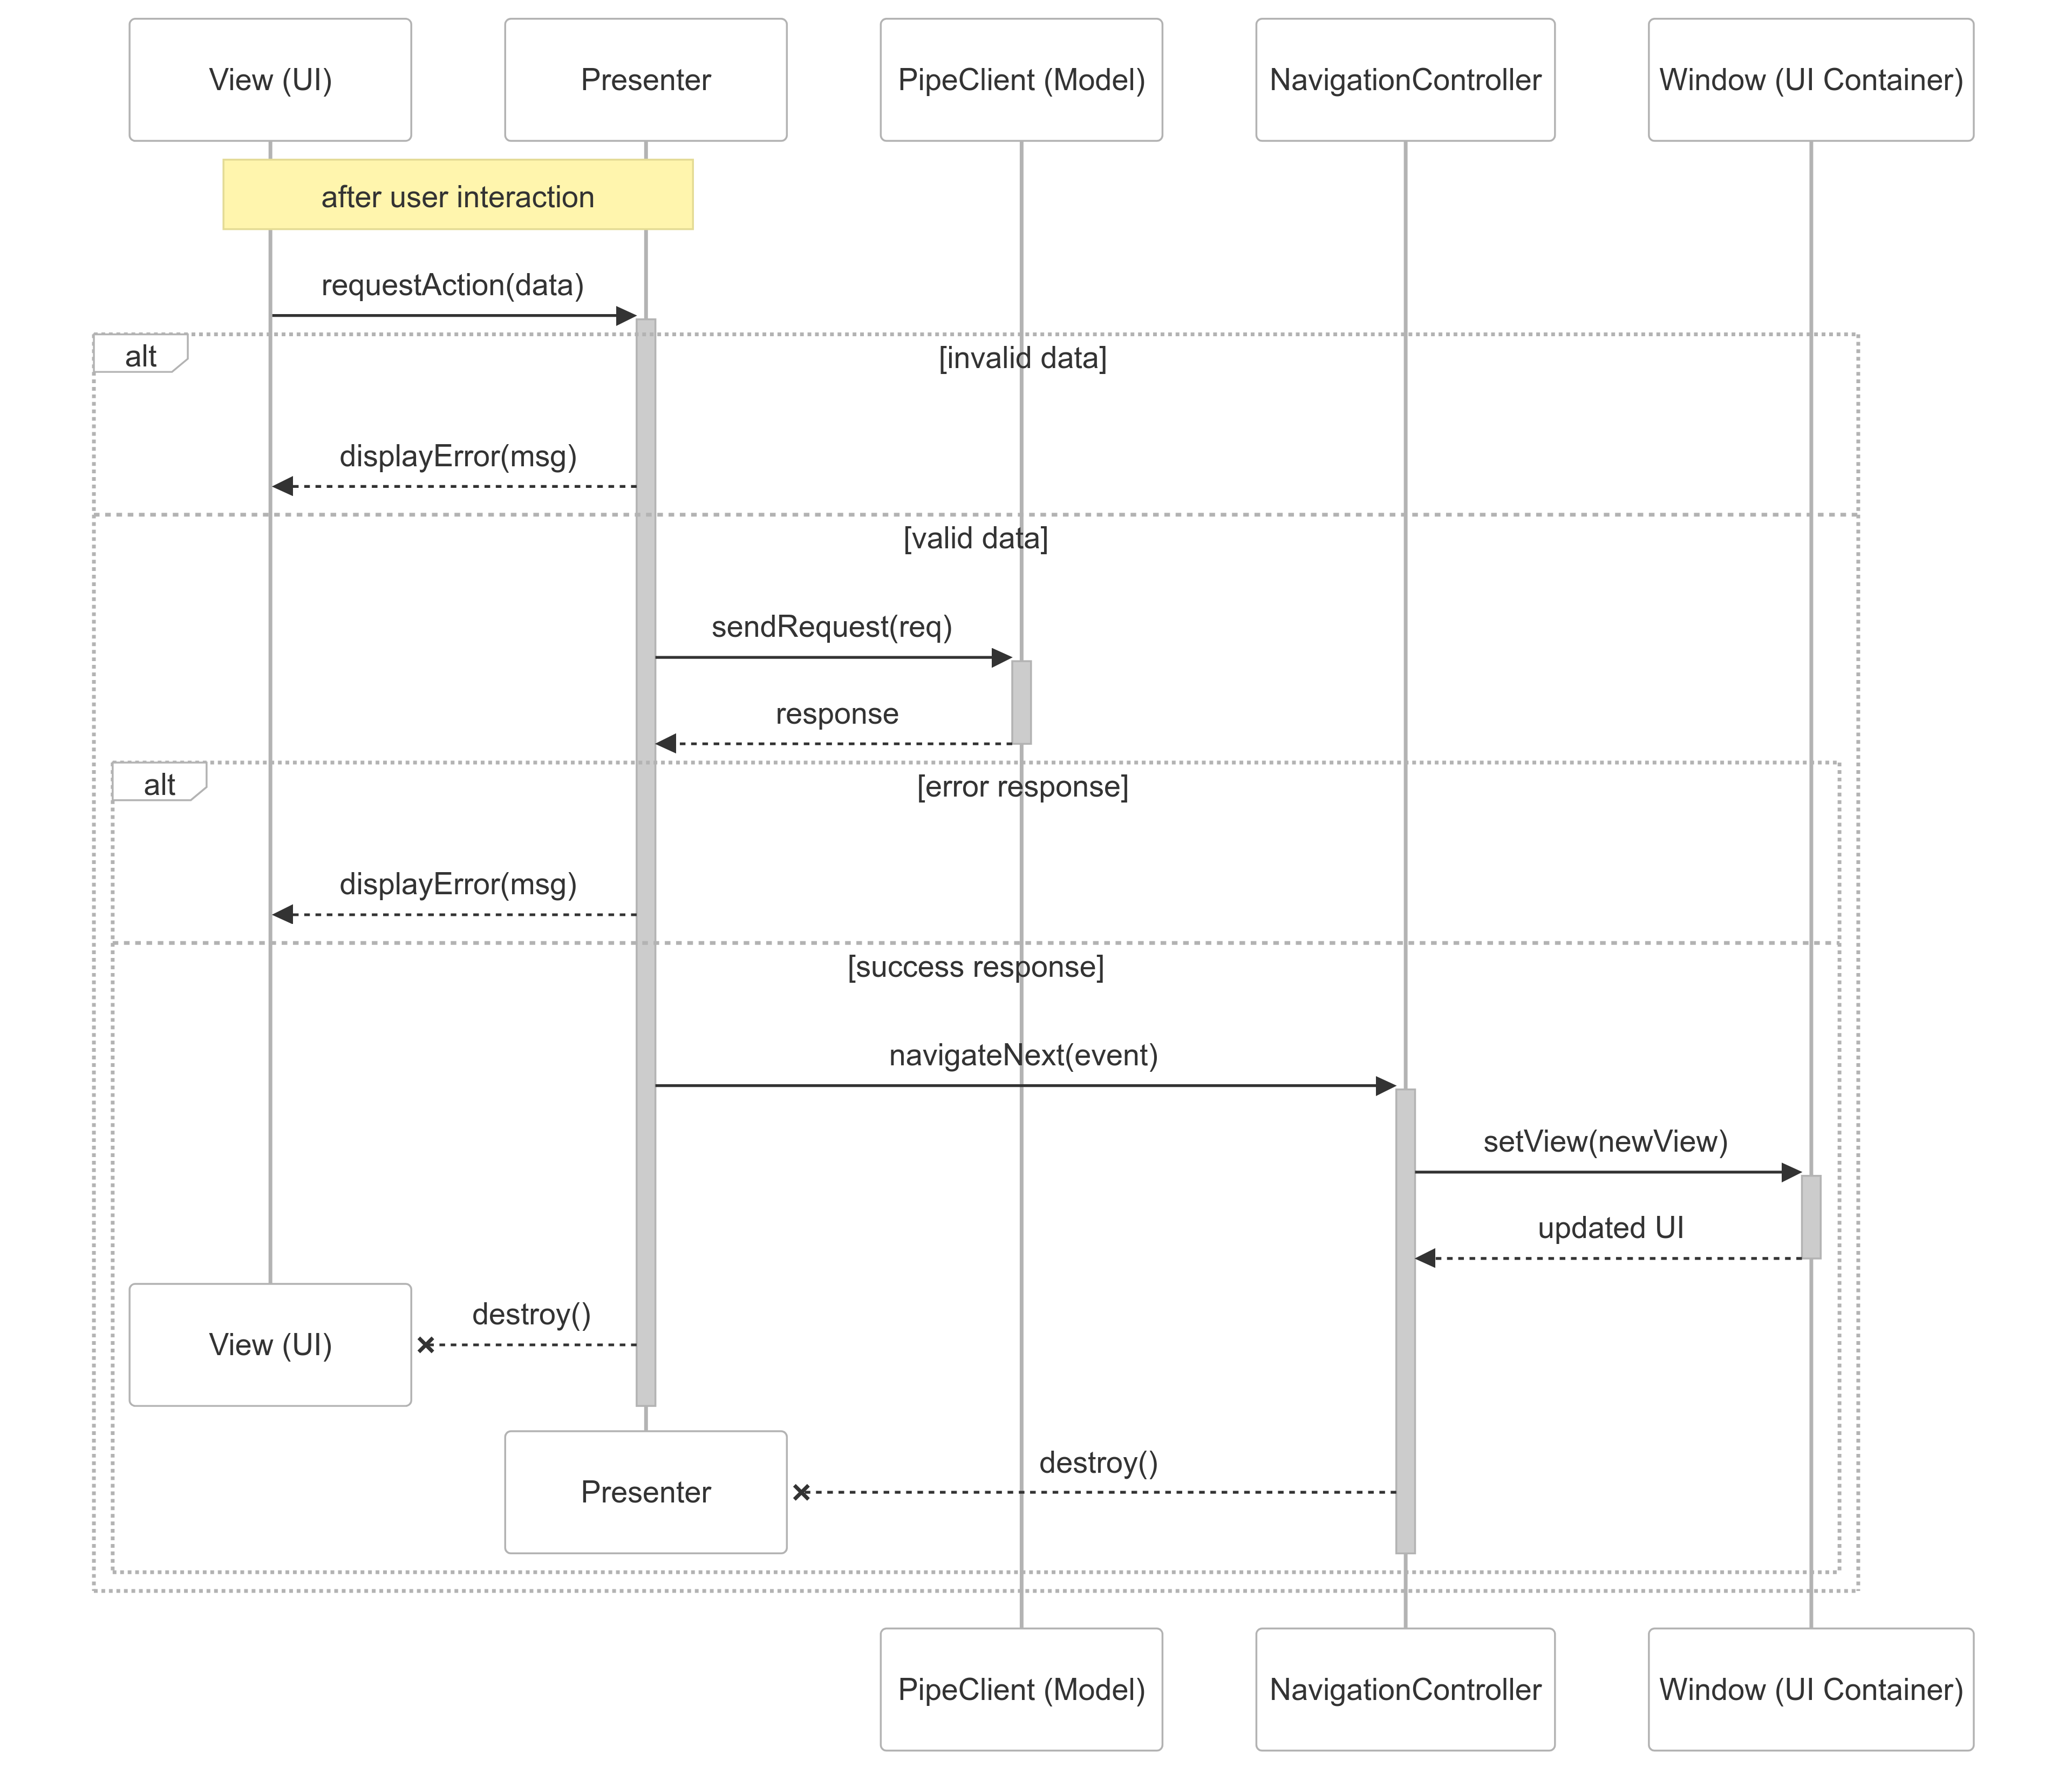
\includegraphics[width=0.9\textwidth]{figures/mvp-diagramma-sequenza.png}
	\caption{Diagramma di sequenza pattern MVP}
	\label{fig:mvp-diagramma-sequenza}
\end{figure}
In figura \ref{fig:mvp-diagramma-sequenza} è possibile visualizzare i componenti dell'architettura proposta, che trae ispirazione dell'articolo \cite{Ramsdale2010}.
L'immagine offre una rappresentazione delle interazioni che dovrebbero avvenire in una corretta implementazione dell'architettura.

Nell'interfaccia grafica di ClientShield non esiste un vero e proprio Model, i dati da rappresentare risultano essere gli stati della protezione.
Pertanto, a svolgere tale ruolo è \class{PipeClient}, che è il responsabile della comunicazione con il servizio Windows, dal quale ottiene risposte sull'esito delle operazioni e sullo stato della protezione.

Stando a quanto riportato in sezione \ref{sec:casi-d-uso}, le possibili \class{View} sono tre e rispecchiano gli stati di ClientShield: non registrato, protezione attiva, protezione disattivata.
Ognuna di esse dovrà avere il proprio \class{Presenter} che consenta di validare e processare i dati delle richieste utente.

L'architettura proposta sostituisce all'implementazione di una coda di eventi, utilizzata in \cite{Ramsdale2010}, l'utilizzo della classe \class{NavigationController}.
Quest'ultima si configura come un \textit{observer} per i \class{Presenter}, che notificano gli eventi scatenati dall'interfaccia grafica.
Tali eventi, che rappresentano tipicamente il passaggio da uno stato all'altro,  necessitano una visione globale sull'applicazione ed una gestione centralizzata, compito che, pertanto, non può essere svolto da un semplice \class{Presenter}.

%---------------------------------------------------
% CAPITOLO 4
%---------------------------------------------------

\chapter{Implementazione}

La successiva, ed ultima, fase del progetto ha riguardato lo sviluppo, che ha compreso la scelta delle tecnologie da utilizzare e l'effettiva scrittura di codice.
Questa fase è stata indubbiamente resa più veloce e diretta grazie all'attento lavoro di documentazione, analisi e progettazione descritto nei capitoli precedenti.

\section{Scelta del linguaggio}

Il linguaggio scelto per lo sviluppo di ClientShield è stato \cs con .NET 8.
Questa scelta è stata piuttosto naturale, sia perché è lo stesso linguaggio utilizzato dalla precedente implementazione sviluppata da FlashStart, ma soprattutto grazie alle caratteristiche del linguaggio, che si adeguano perfettamente ai requisiti del software.
Innanzitutto \cs è un linguaggio moderno, che consente uno sviluppo ed una manutenzione più semplici, grazie alla sua sintassi chiara e funzionalità avanzate.
L'utilizzo di questo linguaggio garantisce un ottimo equilibrio tra efficienza e semplicità, garantendo una gestione automatica della memoria tramite la garbage collection\footnote{La \textbf{garbage collection} identifica e recupera automaticamente la memoria occupata da oggetti non più utilizzati, evitando che il programma esaurisca lo spazio disponibile.} ed una vasta disponibilità di librerie e framework che facilitano lo sviluppo.

Analogamente a Java, \cs supporta la programmazione multi-platform, ma risulta più adatto per ClientShield grazie alla perfetta integrazione dell'ecosistema .NET con Windows, che rappresenta il target principale del software.
\cs, infatti, ha accesso facilitato alle API di Windows grazie a librerie ufficiali sviluppate da Microsoft, che fornisce inoltre guide e documentazione utili all'implementazione e installazione di servizi Windows sviluppati in .NET. 

Il linguaggio supporta anche l'implementazione di interfacce utente native attraverso \gls{WPF}, che permette l'applicazione del pattern \gls{MVP} scelto in fase di analisi.
Inoltre la comunicazione tramite named pipes è supportata nativamente e vengono offerti diversi strumenti per la creazione di un installer.
Ciò consente l'uso del medesimo linguaggio per tutti i progetti definiti in sezione \ref{ssec:organizzazione-sotto-progetti}, garantendo coerenza all'intera codebase, oltre a permettere una struttura assolutamente simile a quella prevista.

La scelta del linguaggio conduce all'ovvia adozione di Visual Studio come \gls{IDE}\footnote{Un \textbf{\gls{IDE}} è un software che fornisce strumenti come editor di testo, compilatori e debugger per facilitare la scrittura e la gestione del codice.}, che offre suggerimenti di codice, editor integrato di interfacce utente, ottimi strumenti di debugging, supporto per il version control di Git e tantissime altre funzionalità che lo rendono una scelta ottima per questo linguaggio.

La directory di ClientShield segue la struttura illustrata in figura \ref{fig:struttura-directory-clientshield}, è stata creata un'unica soluzione composta da tre dei quattro progetti previsti:
\begin{itemize}
	\item \textbf{Service:}
	è un progetto di tipo Worker Service, template presente in Visual Studio e adatto allo sviluppo di un servizio Windows.
	
	\item \textbf{Client:}
	è un progetto di tipo \gls{WPF}, adatto allo sviluppo di una moderna interfaccia grafica per sistemi Desktop.
	
	\item \textbf{Common:}
	questo progetto contiene i messaggi e le configurazioni della comunicazione inter-processo, utilizzabili sia da Service che da Client.
\end{itemize}
L'installer non è stato sviluppato nella versione prototipale.

\section{Tecnologie di supporto}

\subsection*{NuGet}

Per lo sviluppo di ClientShield sono state utilizzate diverse librerie esterne, perciò, allo scopo di gestire le dipendenze del progetto, è stato utilizzato NuGet\footnote{Sito ufficiale NuGet: \url{http://nuget.org}}, il gestore di pacchetti ufficiale per l'ecosistema .NET.

NuGet permette di aggiungere, aggiornare e rimuovere pacchetti esterni con facilità, evitando la necessità di includere manualmente le librerie.
Ha un ruolo chiave nel processo di sviluppo, in quanto, grazie al controllo di versione sulle dipendenze, segnala problemi di incompatibilità tra le librerie di un progetto, evitando potenziali errori difficili da individuare manualmente.

\subsection*{Git}

Per lo sviluppo è stato fondamentale l'utilizzo di Git\footnote{Sito ufficiale di Git: \url{http://git-scm.com}}, un sistema di versionamento, che permette un efficace controllo sulle modifiche, consentendo di preservare l'integrità del codice.
Git è senza dubbio uno dei sistemi di versionamento più utilizzati, grazie alla capacita di gestire in modo molto efficiente anche progetti particolarmente complessi.

Il software consente di tenere traccia di ogni modifica apportata al codice, permettendo di ripristinare versioni precedenti in caso di errori o di confrontare diversi stati del progetto. Nel contesto di ClientShield, trattandosi di un prototipo sviluppato da zero, il lavoro si è concentrato prevalentemente su un unico branch principale, evitando la necessità di gestire rami multipli tipici di progetti più strutturati.
Per migliorare la leggibilità dello storico delle modifiche è stata adottata una struttura standardizzata per i commit, preceduti da tag identificativi che ne indicano il tipo: ad esempio i tag \texttt{[DOC]} per la documentazione o \texttt{[NEW]} per le nuove funzionalità.

Un ulteriore vantaggio di Git è la grande compatibilità con piattaforme cloud come GitHub\footnote{Sito ufficiale di GitHub: \url{http://github.com}}, consente di lavorare su computer diversi con codice sempre sincronizzato.

\subsection*{Librerie di gestione JSON}

In fase di analisi si è scelto di utilizzare JSON per la comunicazione inter-processo.
Tale scelta ha reso possibile l'utilizzo di un meccanismo di deserializzazione che avesse un modello di ereditarietà, in modo da poter effettuare un casting intelligente.

A tal scopo è stata utilizzata la libreria JsonSubTypes\footnote{Sito ufficiale JsonSubTypes: \url{http//manuc66.github.io/JsonSubTypes/}}, che consente di definire una classe base comune per tutte le richieste, semplificando la gestione dei messaggi.
Invece di trattare ogni richiesta come entità separata, il sistema utilizza un tipo di richiesta generico, che viene poi convertito in richieste specifiche, ad esempio di autorizzazione o registrazione.
Il controllo e la conversione da messaggio generico a specifico sono gestiti direttamente dalla libreria, eliminando la necessità di controlli manuali sulla struttura delle richieste e migliorando la pulizia del codice.

La serializzazione e la deserializzazione sono gestite attraverso la libreria Newtonsoft.Json\footnote{Sito ufficiale Newtonsoft.Json: \url{http://www.newtonsoft.com/json}}. Questa libreria è in grado di lavorare assieme a JsonSubTypes per la corretta conversione da classe a JSON e viceversa, offrendo semplicità, ottime prestazioni e individuazione automatica di errori di conversione.

\section{Implementazione progetto Service}

Il progetto per l'implementazione del servizio Windows è stato sviluppato a partire dalla guida \cite{MicrosoftServices2021} realizzata da Microsoft.
Il servizio è stato implementato, come suggerito dalla guida, attraverso un \class{BackgroundService} che, all'avvio, instanzia un \class{ServerNamedPipe} e un \class{ProtectionManager}, adeguatamente introdotti nella sezione \ref{ssec:analisi-protezione} ed illustrati in figura \ref{fig:protezione-facade-pattern}.

\paragraph{ServerNamedPipe} è una classe implementata facendo uso delle librerie di sistema e funge da server per la comunicazione inter-processo.
Il server sarà sempre in ascolto sulla pipe di nome "FlashStart-ClientShield-Service-Pipe" finché il servizio Windows è attivo.
Il costruttore necessita il passaggio di un oggetto \class{ProtectionManager}, col quale il server si interfaccia per eseguire i comandi ricevuti dalla named pipe.

\paragraph{ProtectionManager} è la classe responsabile della gestione globale del servizio di protezione, coordinando la comunicazione con le API FlashStart, l'esecuzione del server \gls{DNS} locale e la gestione delle credenziali.
Questa classe funge da punto di raccordo tra le classi che offrono i suddetti servizi:
\begin{itemize}
	\itemdef{CredentialManager:} viene utilizzato all'instanziazione di {ProtectionManager} per controllare l'esistenza di un cliente già registrato.
	Durante le fasi di registrazione e logout questa classe si occupa di salvare o eliminare le credenziali sul dispositivo.
	
	\itemdef{FlashStartClient:} viene utilizzato durante tutta l'esecuzione del servizio per interfacciarsi con le API di FlashStart.
	
	\itemdef{DnsServer:} classe dedicata alla gestione del server \gls{DNS} locale, viene inizializzato da \class{ProtectionManager} all'avvio della protezione.
\end{itemize}

\paragraph {CredentialManager} utilizza il gestore di credenziali Windows per l'archiviazione del Client ID, cioè il codice utente univoco necessario per l'autenticazione con i server FlashStart.
Questa classe è sviluppata come wrapper dell'omonimo modulo appartenente alla libreria Meziantou.Framework.Win32, gestendo automaticamente le configurazioni necessarie per consentire una più facile interazione da parte di \class{ProtectionManager}.
I metodi esposti consentono in particolare la registrazione, l'eliminazione, l'aggiornamento e la visualizzazione (se presente) del codice utente sul dispositivo.\\

\paragraph{FlashStartClient} utilizza un client HTTP fornito dalle librerie di sistema per effettuare richieste ai server FlashStart, impostandone automaticamente l'header di autenticazione.
Questa classe fornisce metodi per permettere di effettuare le richieste di \textit{registrazione}, \textit{autorizzazione} e \textit{check}.

\subsection{Implementazione server DNS}

Il server \gls{DNS} rappresenta il cuore del progetto e la sua implementazione è un aspetto cruciale, poiché le future modifiche del software riguarderanno prevalentemente questa parte.  
È di fondamentale importanza aderire alla struttura proposta in fase di analisi e rendere il codice chiaro ed organizzato, in modo tale da facilitarne la modifiche e, soprattutto, l'estensione.
L'implementazione descritta di seguito segue le linee guida delineate nella sezione \ref{ssec:analisi-server-dns}, sfruttando i pattern progettuali individuati per ottenere gli obiettivi di manutenibilità, estensibilità ed efficienza.

ClientShield utilizza \class{StubbornDnsServer} come server \gls{DNS}.
Questa classe funge da decorator per l'implementazione di base \class{DnsServer}, utilizzando il pattern per estendere le funzionalità del server \gls{DNS}, consentendogli di imporsi come predefinito di sistema.
Per consentire l'operazione, \class{StubbornDnsServer} si avvale dei metodi esposti dalla classe \class{NetworkManager}, responsabile della gestione delle impostazioni di rete.  

\paragraph{NetworkManager} è una classe statica che si occupa della configurazione del \gls{DNS} del dispositivo.
Interfacciandosi direttamente con le librerie di sistema di Windows, \class{NetworkManager} consente di impostare il \gls{DNS} su uno specifico indirizzo statico e di ripristinarlo alla modalità automatica quando necessario.
Il codice prodotto sfrutta la libreria \textit{System.Management} per interagire direttamente con il sistema operativo.
Questa libreria consente di configurare gli indirizzi dei server \gls{DNS} utilizzati per la risoluzione dei domini.
La soluzione proposta imposta come unico indirizzo valido l'IP 127.0.0.1, dove opera il server gestito da ClientShield.

\paragraph{StubbornDnsServer} estende i metodi \textit{start} e \textit{stop} dell'implementazione di base per gestire correttamente la configurazione del \gls{DNS} di sistema.
All'avvio del server locale, \class{StubbornDnsServer} utilizza l'evento \textit{NetworkChange}, appartenente alle librerie di sistema, per monitorare ogni cambiamento alle configurazioni di rete e assicurarsi costantemente che il server \gls{DNS} rimanga impostato correttamente.
All'arresto, la gestione dell'evento viene disattivata e il \gls{DNS} viene ripristinato alla modalità dinamica, garantendo che il sistema torni al suo stato originale.\\

L'implementazione del server \gls{DNS} di base segue uno sviluppo molto modulare, sfruttando varie componenti che ne consentono la facile estensione e modifica.
Non solo, lo sviluppo modulare consente di suddividere i compiti da svolgere in routine eseguibili da thread in concorrenza, rendendo la risoluzione dei domini più efficiente.
Il server necessita di due componenti fondamentali:
\begin{itemize}
	\itemdef{DnsResolver:} interfaccia di risoluzione delle richieste \gls{DNS}.
	\itemdef{SocketListener:} interfaccia di gestione di un socket, consente di attendere richieste su una porta ed eventualmente rispondere.
\end{itemize}
Tali componenti, oltre a garantire flessibilità al sistema, contribuiscono anche a mantenere il codice della classe \class{DnsServer} più semplice e, dunque, facile da manutenere.

Al suo avvio il server utilizza la classe \class{TaskFactory}, appartenente alle librerie di sistema, per schedulare l'esecuzione parallela dei task di ascolto e risoluzione delle richieste \gls{DNS}.
Queste routine sono svolte per un periodo di tempo indefinito, infatti, fintanto che il servizio non riceve una richiesta di stop dal server named pipe o il computer non viene spento, il server deve procedere con la sua esecuzione.
Per questo motivo entrambi i task sono creati specificando alla \class{TaskFactory} il parametro \textit{LongRunning}, ciò assicura che abbiano ambedue dei thread dedicati, prevenendo l'uso di quelli appartenenti al ThreadPool, riservati ai task di breve durata.
Per gestire in maniera ottimale la concorrenza causata dai task, il server mantiene una coda di messaggi bloccante.
La coda consente a \class{SocketListener} e \class{DnsResolver} di cooperare tra loro in modo sicuro, evitando race conditions.

La routine di ascolto delle richieste è completamente affidata alla classe \class{UdpListener}, un'implementazione dell'interfaccia \class{SocketListener} che utilizza il client UDP delle librerie di sistema per monitorare la porta 53, dedicata alle comunicazioni \gls{DNS}.
Infatti, come riportato in \cite{RFC1035}: ``I messaggi inviati utilizzando UDP usano la porta server 53 (decimale). [...] UDP non è accettabile per i trasferimenti di zona, ma è il metodo raccomandato per le query standard su Internet.''.

Alla ricezione di una richiesta \gls{DNS}, \class{UdpListener} la aggiunge alla coda di messaggi.
Ciò consente di rendere il thread di ascolto sempre reattivo, in quanto scaricato di qualsiasi lavoro di gestione della richiesta, minimizzando i tempi di reazione alla ricezione.


La routine di risoluzione del dominio fa uso della classe \class{DoHResolver}, cioè un'implementazione dell'interfaccia \class{DnsResolver} che utilizza il client HTTP delle librerie di sistema per inviare richieste di risoluzione \gls{DNS} ai server FlashStart.
La classe si occupa di assicurarsi che venga utilizzata la versione 2 di HTTP, garantendo la crittografia della comunicazione.
La classe espone un metodo per la risoluzione dei domini: la richiesta viene redirezionata ai server FlashStart fornendo il client ID, che verrà utilizzato per l'applicazione del filtro.
La risposta ottenuta può contenere l'indirizzo IP corrispondente al dominio richiesto o, in caso di blocco, una stop page indicante il motivo della restrizione.  

La risoluzione del dominio da parte del server prevede tre fasi:
\begin{enumerate}
	\item Prima di essere affidata al resolver, il nome del dominio viene estrapolato dalla richiesta, permettendo l'eventuale esclusione di domini specifici dal filtro.
	A tal scopo viene utilizzata la libreria ARSoft.Tools.Net\footnote{Sito ufficiale ARSoft.Tools.Net: \url{https://github.com/alexreinert/ARSoft.Tools.Net}}, che offre efficaci strumenti per una decodificazione veloce di richieste \gls{DNS}.
	
	\item Decodificato il dominio, se appartenente alla lista dei domini esclusi dal filtro, la richiesta viene risolta utilizzando un server \gls{DNS} pubblico, altrimenti viene utilizzato \class{DoHResolver} per la risoluzione.
	
	\item Una volta ottenuta la risposta dal server \gls{DNS} esterno, viene inviata al processo che aveva richiesto la risoluzione.
\end{enumerate}
Infine, all'arresto, il server si occupa di interrompere correttamente l'esecuzione parallela dei task.

\section{Implementazione progetto Client}

Sebbene si sia discusso del possibile sviluppo di un'interfaccia grafica multi-piattaforma, il prototipo di ClientShield utilizza la libreria \gls{WPF}, specifica per ambienti Windows.
La scelta è motivata principalmente dalla maggiore familiarità con la libreria, che offre un'ottima integrazione con .NET.
Tuttavia, è doveroso sottolineare che il progetto segue l'architettura software analizzata in sezione \ref{ssec:analisi-mvp}.
Pertanto le modifiche necessarie per un eventuale sviluppo multi-platform riguarderanno la semplice sostituzione delle classi strettamente riguardanti l'interfaccia grafica, ossia le \class{View}.
Inoltre è opportuno sottolineare che, grazie ad una corretta aderenza al pattern \gls{MVP}, tali modifiche sono da considerarsi semplici e di impatto minore, in quanto la totale passività della parte visiva ha concesso di spostare l'intera logica all'interno delle classi \class{Presenter}.

L'obiettivo di quest'implementazione non è soltanto agevolare uno sviluppo multi-platform, ma anche garantire la modifica dell'interfaccia con il minimo intervento.
Ciò facilita la correzione dell'aspetto grafico, che risulta soltanto abbozzato nell'implementazione prototipale, in quanto poco interessante dal punto di vista ingegneristico, ma che è cruciale per uno sviluppo business.
\begin{figure}[H]
	\centering
	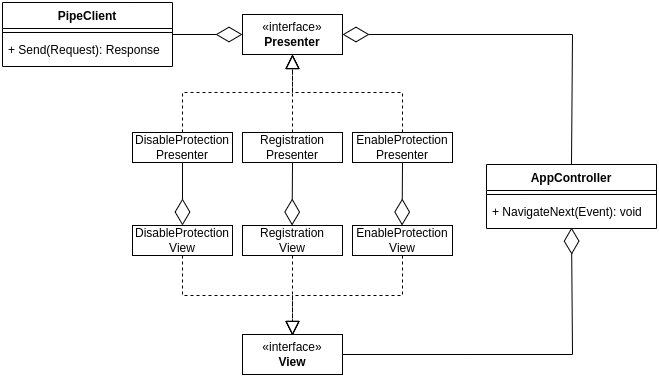
\includegraphics[width=1.0\textwidth]{figures/mvp-classes.png}
	\caption{Struttura delle classi dell'interfaccia grafica}
	\label{fig:mvp-struttura-classi}
\end{figure}
In figura \ref{fig:mvp-struttura-classi} viene illustrata la struttura delle classi.
L'applicazione è strutturata su tre schermate principali e segue la logica illustrata in figura \ref{fig:schema-casi-uso}:
\begin{itemize}
	\itemdef{Schermata di registrazione:} è la schermata dedicata al form di registrazione del dispositivo.
	Deve essere visualizzabile quando non esiste già un utente FlashStart sul dispositivo e permettere l'inserimento dei campi riguardanti la chiave di profilo e il nome del dispositivo.
	
	\itemdef{Schermata di abilitazione della protezione:} è una semplice schermata visualizzabile quando il dispositivo ha già un utente FlashStart registrato, ma la protezione è disattivata.
	Nell'implementazione prototipale contiene due bottoni: uno per l'attivazione della protezione, l'altro per cancellare l'utente dal dispositivo, riportando necessariamente l'applicazione alla schermata di registrazione.
	
	\itemdef{Schermata di disabilitazione della protezione:} è una schermata visualizzabile quando il dispositivo ha già un utente FlashStart registrato e la protezione è attiva.
	La schermata deve presentare un campo per l'inserimento del PIN di disabilitazione (visualizzabile dalla piattaforma cloud) ed un bottone per eseguire la richiesta di disabilitazione.
	Se il codice è corretto la protezione viene disattivata.
\end{itemize}
La struttura di ognuna di queste schermate è definita attraverso il linguaggio XAML implementato da WPF.
Ciò permette di creare le schermate definendo la loro struttura tramite la semplice sintassi offerta dal linguaggio di markup, che consente di legare la schermata XAML a una classe code-behind\footnote{Una classe \textbf{code-behind} è una classe \cs associata a un file XAML che gestisce eventi e logica dell'interfaccia utente, permettendo l'interazione diretta con i controlli definiti nel XAML.} specifica.
Questo consente alla classe associata di interagire direttamente con gli elementi definiti nello XAML senza doverli dichiarare esplicitamente nel codice.

Per ognuna delle suddette schermate sono state realizzate delle specifiche classi \class{View}, responsabile della visualizzazione e \class{Presenter}, responsabile della presentazione dei dati da visualizzare.

\paragraph{View} è il gruppo di classi code-behind corrispondenti alle schermate XAML.
Ogni \class{View} è implementata estendendo la classe \class{UserControl} fornita da \gls{WPF}, che permette di definire gruppi di elementi presenti in una schermata, consentendo di utilizzare la stessa finestra per mostrare schermate differenti.
Ogni \class{View} ha il solo scopo di raccogliere input dall'utente e trasmetterli al proprio \class{Presenter}.
La validazione dei dati è completamente effettuata da quest'ultimo, che, in caso di errore notifica alla \class{View} un messaggio da mostrare all'utente.

\paragraph{Presenter} è il gruppo di classi che gestiscono la logica di presentazione di ciascuna schermata.
Ogni \class{Presenter} si occupa di validare gli input ottenuti dalla \class{View} e di trasmetterli alla classe \class{PipeClient} per l'elaborazione della richiesta inter-processo.
In caso di un qualsiasi errore, il \class{Presenter} si occupa della creazione di un messaggio per permettere alla \class{View} di mostrare la causa all'utente.
Se l'operazione ha avuto successo, invece, notifica l'evento avvenuto alla classe \class{AppController}, che gestirà eventualmente il cambio di schermata.

\paragraph{AppController} è la classe dedicata alla logica di navigazione dell'applicazione. 
La funzione è implementata attraverso il metodo \textit{NavigateNext}, chiamato quando si verifica un evento che cambia lo stato del sistema, come l'inizializzazione, la registrazione o l'attivazione/disattivazione della protezione.
\class{AppController} al verificarsi di un evento cambia adeguatamente le schermata visibile, instanziando la corretta \class{View} con il relativo \class{Presenter} e interagendo con la finestra dell'applicazione.

\paragraph{PipeClient} è la classe responsabile della comunicazione con il servizio Windows.
All'avvio dell'applicazione si connette come client sulla named pipe dedicata a ClientShield, permettendo l'invio dei comandi per la registrazione, autorizzazione e verifica dello stato della protezione, occupandosi della serializzazione e deserializzazione dei messaggi.\\

In figura \ref{fig:schermate-app} è visibile un'anteprima dell'interfaccia utente di ClientShield.
Sono rappresentate le schermate di gestione della protezione (disabilitazione/abilitazione) e di registrazione.
\begin{figure}[H]
	\centering
	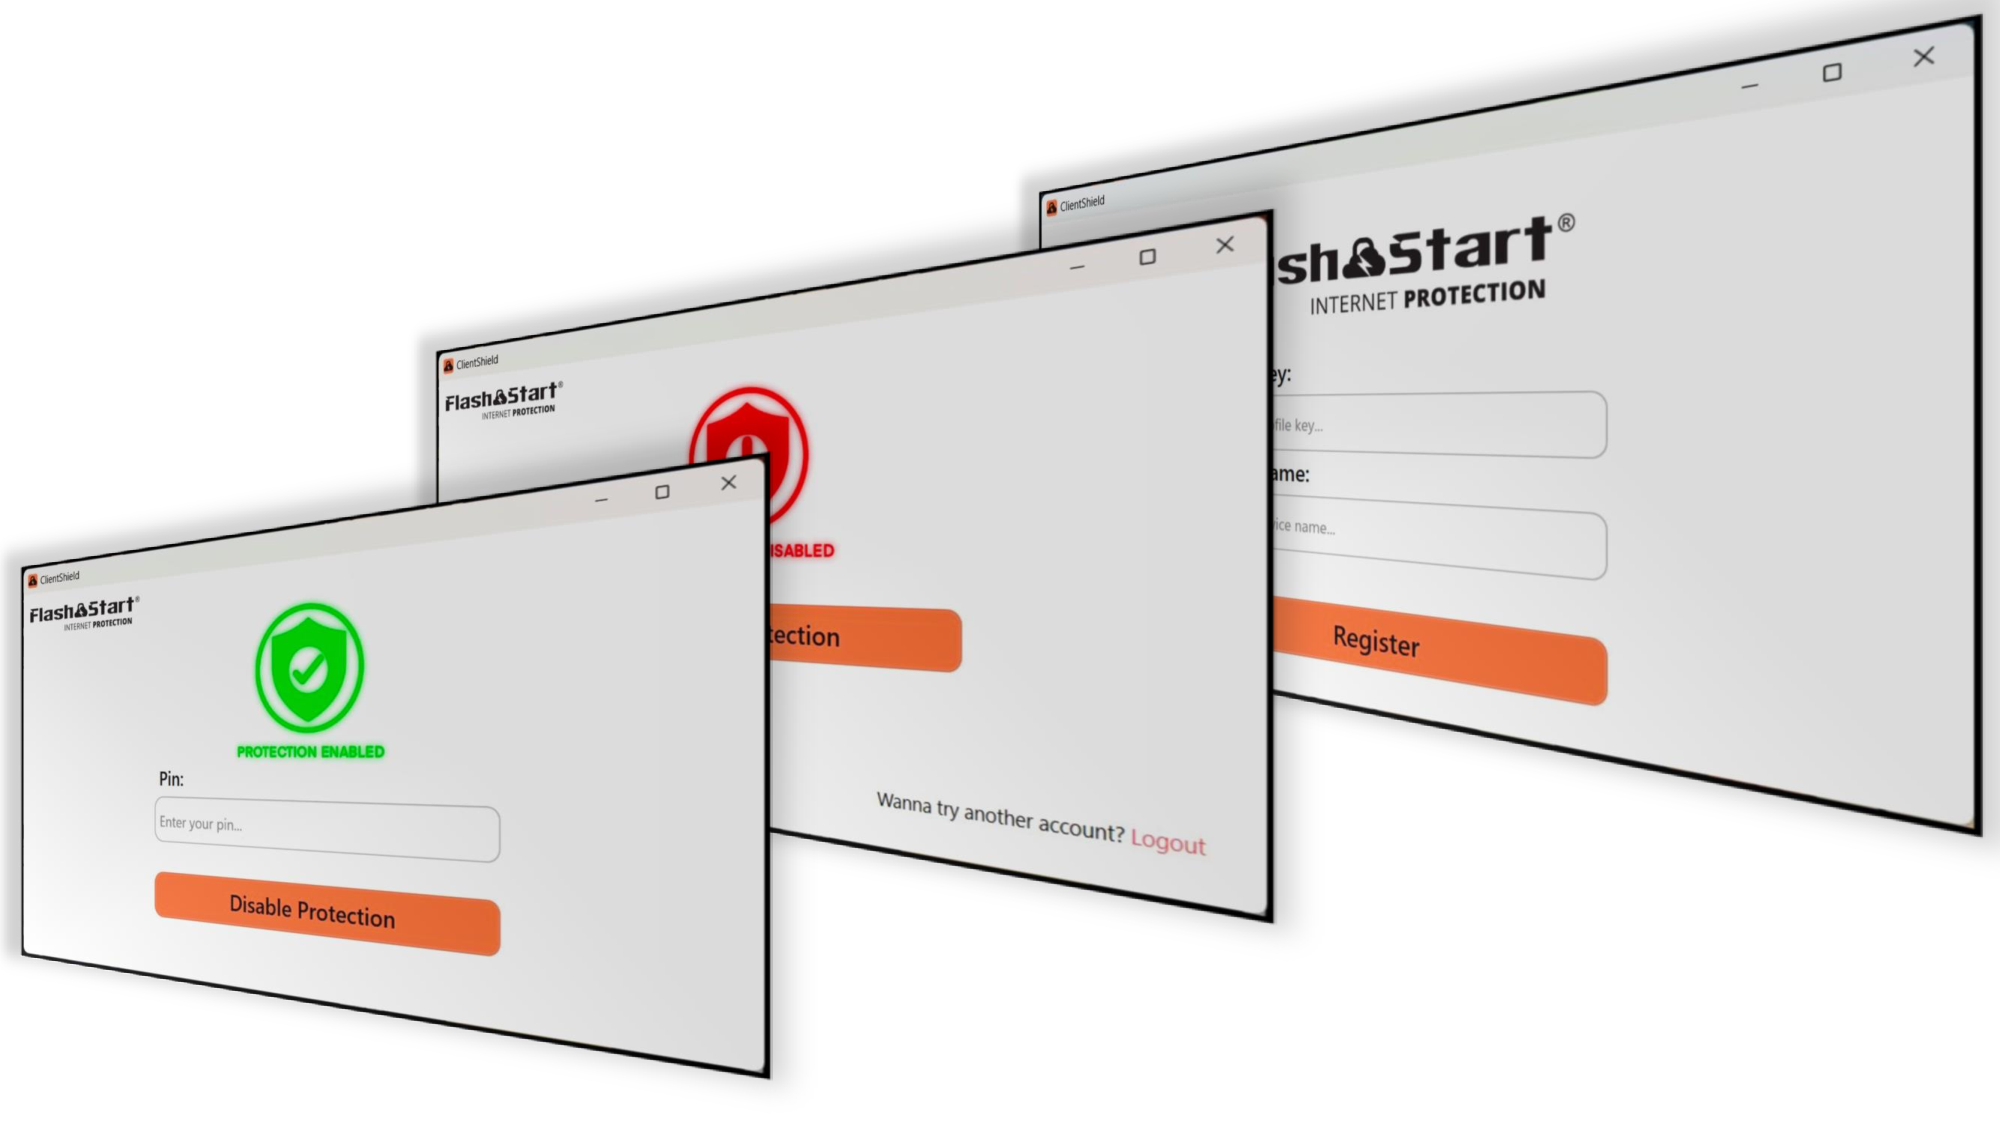
\includegraphics[width=1.0\textwidth]{figures/schermate.pdf}
	\caption{Interfaccia utente ClientShield}
	\label{fig:schermate-app}
\end{figure}


\section{Validazione}

Al termine dello sviluppo, il servizio Windows è stato installato tramite PowerShell per consentire il testing manuale di tutte le funzionalità disponibili.
I test si sono concentrati principalmente sulla verifica del corretto funzionamento del servizio di filtraggio, assicurandone la conformità ai requisiti funzionali.
Tuttavia, una volta appurato il corretto funzionamento del prototipo, sono stati prodotti dei dati quantitativi sull'efficienza del filtro.

Per lo svolgimento dei test è stato utilizzato il sistema \gls{WSL}, che ha permesso di eseguire script Bash in ambiente Windows.
I test sono stati eseguiti su un computer con CPU Intel(R) Core(TM) i5-10210U da 1.60GHz e 8GB di memoria RAM, connesso ad internet tramite cavo ethernet.

La raccolta dei dati è stata effettuata mediante uno script bash che esegue il comando \texttt{dig} per visualizzare i tempi di risposta del \gls{DNS} di sistema sui primi mille domini appartenenti ad una lista online\footnote{Lista di domini utilizzata: \url{https://github.com/fgont/domain-list/blob/master/majestic-domains.txt}}.
Lo script calcola il tempo di risposta medio, minimo e massimo, fornendo informazioni anche sul numero di query perse.
La sua esecuzione è avvenuta inizialmente configurando il DNS statico sull’indirizzo 1.1.1.1, il server pubblico di Cloudflare\footnote{Sito ufficiale Cloudflare: \url{https://www.cloudflare.com}}. Successivamente, è stata attivata la protezione tramite ClientShield, testando sia la nuova implementazione basata su \gls{DoH} sia la versione precedente, che utilizza una \gls{VPN}.
In ognuno dei tre scenari sono stati attivati cinque diversi processi in background che hanno eseguito lo script e trascritto i risultati su dei file di log.
I dati finali dei test sono riportati nella tabella \ref{tab:dns-tests}.

\begin{table}[h]
	\centering
	\renewcommand{\arraystretch}{1.3} % Spaziatura tra le righe
	\setlength{\tabcolsep}{10pt} % Spaziatura tra le colonne
	\begin{tabular}{lcccc}
		\toprule
		\textbf{Test} & \textbf{T.Medio (ms)} & \textbf{T.Min (ms)} & \textbf{T.Max (ms)} & \textbf{Query Perse} \\
		\midrule
		\multicolumn{5}{c}{\textbf{DNS Statico: Cloudflare (1.1.1.1)}} \\
		\midrule
		Test 1 & 67 & 0 & 3999 & 8 \\
		Test 2 & 62 & 0 & 1052 & 8 \\
		Test 3 & 70 & 0 & 2009 & 8 \\
		Test 4 & 65 & 0 & 2888 & 8 \\
		Test 5 & 69 & 0 & 3991 & 8 \\
		\midrule
		\multicolumn{5}{c}{\textbf{DNS con ClientShield DoH Attivato}} \\
		\midrule
		Test 1 & 65 & 19 & 1630 & 8 \\
		Test 2 & 65 & 10 & 1630 & 8 \\
		Test 3 & 65 & 20 & 1620 & 8 \\
		Test 4 & 65 & 20 & 1620 & 8 \\
		Test 5 & 66 & 20 & 1639 & 8 \\
		\midrule
		\multicolumn{5}{c}{\textbf{DNS con ClientShield VPN Attivato}} \\
		\midrule
		Test 1 & 98 & 9 & 1647 & 8 \\
		Test 2 & 102 & 9 & 1922 & 8 \\
		Test 3 & 102 & 18 & 1922 & 8 \\
		Test 4 & 102 & 9 & 1922 & 8 \\
		Test 5 & 102 & 9 & 1932 & 8 \\
		\bottomrule
	\end{tabular}
	\caption{Risultati dei test sul tempo di risposta DNS}
	\label{tab:dns-tests}
\end{table}
Questi test presentano alcune limitazioni, poiché sono stati eseguiti su un numero limitato di iterazioni e su un'unica macchina.
Tuttavia sono ritenuti sufficienti a verificare il buon funzionamento del prototipo, che fornisce risposte in tempi, in media, simili ad uno dei \gls{DNS} più utilizzati al mondo e sempre minori rispetto alla precedente implementazione.
I tempi di risposta pari a 0ms registrati nei test con il \gls{DNS} di CloudFlare sono probabilmente dovuti all'utilizzo della cache, una funzionalità non implementata nel prototipo di ClientShield.
La differenza tra i tempi massimi di risposta è invece dovuta, presumibilmente, a diverse configurazioni tra il \gls{DNS} pubblico e quello realizzato in questa tesi.
Nella tabella è inoltre riportata la perdita sistematica di otto query per tutti i \gls{DNS} utilizzati, ciò è dovuto alla lista di domini sfruttata.
L'ultimo aggiornamento della lista è, infatti, datato 2017 al momento della scrittura di questa tesi.
Alcuni dei domini utilizzati non esistono più, ad esempio l'indirizzo storify.com apparteneva ad un social network chiuso nel 2018.

\chapter{Conclusioni e sviluppi futuri}

L'implementazione del software ClientShield proposta in questa tesi vede una completa revisione del suo predecessore.
Il lavoro sviluppato in questa tesi realizza uno sviluppo alternativo, che non si limita al semplice passaggio di tecnologia da \gls{VPN} a \gls{DoH} o alla soddisfazione dei requisiti richiesti dall'azienda.
Il sistema sviluppato adotta una visione a lungo termine, non solo soddisfacendo i requisiti richiesti, ma garantendo anche un'architettura facilmente estendibile per futuri sviluppi.

I pattern proposti si sono rivelati fondamentali, permettendo una corretta separazione dei concetti del dominio e proponendo una struttura altamente modulare e organizzata.
Ciò consente una semplice manutenzione del progetto e permette di estendere il software con minimi interventi mirati, incontrando perfettamente le necessità aziendali.
Infatti, sebbene il lavoro svolto abbia prodotto risultati positivi, è necessario ricordare che la tesi tratta un'implementazione prototipale, che dovrà necessariamente essere oggetto di revisione da parte di FlashStart per un effettivo impiego in ambiente business.

La realizzazione del progetto ha inoltre permesso di esplorare una soluzione di filtraggio alternativa, che sfrutta un server \gls{DNS} locale piuttosto che una scheda di rete virtuale.
Ciò ha dimostrato non soltanto il funzionamento della soluzione, ma anche la sua potenziale efficienza, che, nei test effettuati, supera la precedente implementazione.

Per quanto riguarda gli sviluppi futuri, ClientShield dovrà sicuramente essere esteso aggiungendo le funzionalità mirate all'implementazione business e non riguardanti il sistema prototipale.
Un aspetto fondamentale per il futuro sviluppo sarà la revisione della gestione degli errori, introducendo funzionalità avanzate di logging, attualmente non approfondite nell'implementazione prototipale.  
Sarebbe interessante inoltre aggiungere funzionalità di caching, che permetterebbero al sistema dei tempi di risposta nettamente minori quando, ad esempio, si navigano più pagine di uno stesso sito.
Infine, un ultimo aspetto rilevante sarebbe la valutazione di un'effettiva implementazione multi-platform, che estenderebbe il funzionamento del progetto anche ad altri sistemi operativi, ampliandone le potenzialità.  


%----------------------------------------------------------------------------------------
% BIBLIOGRAPHY
%----------------------------------------------------------------------------------------

\backmatter

\bibliographystyle{alpha}
\bibstyle{alpha}
\bibliography{bibliography}

\begin{acknowledgements} % this is optional
Al termine di questa tesi desidero, innanzitutto, ringraziare il mio relatore Mirko Viroli e il mio correlatore Nicolas Farabegoli, che hanno seguito con attenzione e grande disponibilità l'intero processo di produzione di questo elaborato, a partire dalla scelta dell'argomento.

Ci tengo inoltre a ringraziare Francesco Collini, CEO di FlashStart, per avermi non soltanto dato l'opportunità di sviluppare questo appassionante progetto, ma anche per avermi offerto supporto ed incoraggiamento quando serviva.
Insieme a lui non posso non ringraziare gli altri colleghi di FlashStart, che mi hanno affiancato durante il tirocinio e lo sviluppo della tesi, rendendo il cammino decisamente più leggero.

Ringrazio tanto tutti i miei amici di Fano, tutti quelli che mi sono vicini da anni e che hanno reso l'intero percorso di studi stupendo, non soltanto fatto di libri, ma di legami.
Di qualsiasi momento passato insieme ho nostalgia.

Un grande grazie agli amici dell'università, con cui ho sostenuto esami, progetti e bellissime giornate.
Senza i quali il campus è decisamente più triste e grazie ai quali ho a cuore Cesena come se fosse la mia città.

Ringrazio poi Federica e Martina, i cui nomi non potevano essere semplicemente mischiati nel gruppo.
Grazie di cuore per l'interesse dimostrato in questi anni, per esserci state, anche solo con una semplice parola, con un messaggio o con un abbraccio quando serviva.

Un grandissimo grazie a Matilde, che in questi tre anni mi ha accompagnato mano nella mano fino a al raggiungimento di questo traguardo.
Qualche riga non basta per riconoscere il valore dei piccoli gesti, delle belle parole e dei sentimenti dimostrati fino ad oggi.

Un grazie dal cuore a Javid, gemello più che amico, con cui ho condiviso ogni singola esperienza, studi, amicizie, gioie e la cui presenza è una certezza costante da quando eravamo bambini.
Terminata questa tesi, a malincuore prendo coscienza del fatto che il percorso di studi assieme è terminato, ma ricordo di quando, con le mani piccole piccole digitavo il tuo numero sul telefono di casa, che ancora ricordo a memoria, e stavamo in chiamata ore.
Confido che, anche se le nostre strade, magari, si separeranno e saremo troppo distanti per vederci, non ci scorderemo di restar bambini quel tanto che basta per sentirci ancora, a parlare di niente per ore.

A Valentina, Matteo, Filippo e Martina, devo, non solo questo piccolo successo, ma l'intera vita.
Tutto ciò che ho imparato da voi tutti è indescrivibile, tutto ciò che vi devo è inimmaginabile.
Il sangue, da solo, non basta a tenere legata la famiglia, ciò che fa la differenza è la certezza che, nonostante la distanza, nonostante tutto, possiamo sempre contare l'uno sull'altro.
Vivendo assieme ho senza dubbio imparato che l'amore va oltre le differenze, oltre le difficoltà e unisce in un legame unico, assoluto e indissolubile, che è l'unica ragione che trovo se cerco di spiegarmi come abbiamo fatto ad attraversare certi momenti della nostra vita.
In questo momento in cui a poco a poco, ognuno di noi sta prendendo la sua strada, desidero augurarci il meglio.

Ringrazio il mio papà, che, nonostante le poche parole e i suoi strani modi di dimostrare affetto, in fondo so essere fiero di me.
Ricordo senza dubbio e con molto calore quando da bambino correvo nel letto arrabbiato e tu ti sedevi sul bordo a consolarmi, accarezzandomi la testa con i tuoi manoni.

Mi si stringe il cuore mentre ringrazio la mia mamma, che non ha mai mancato di farmi sentire tutto il suo immenso amore.
Non ricordo nemmeno un giorno della mia vita in cui, entrando dentro casa, non sono stato accolto da un tuo abbraccio.
Non esiste un mio traguardo che tu non abbia celebrato e non esiste gioia se non posso condividerla con te.
Ogni carezza, ogni bacio ed ogni abbraccio rimarranno per sempre impressi nella mia memoria.

Infine, vorrei lasciare un piccolo spazio in fondo per ringraziare la mia nonna, il cui amore e orgoglio sento attraversare il tempo e raggiungermi.



\end{acknowledgements}

\end{document}